%%========================================================================
%% LaTeX scriptiesjabloon
%%========================================================================


%%========================================================================
%% Preamble
%%========================================================================

\documentclass[pdftex,a4paper,12pt,twoside]{report}

%%---------- Extra functionaliteit ---------------------------------------
\usepackage{tipa}								% phonetics
\usepackage[utf8]{inputenc}						% Accenten gebruiken in tekst (vb. é ipv \'e)
\usepackage{amsthm}								% Theorum package
\usepackage{amsfonts}        					% AMS math packages: extra wiskundige
\usepackage{amsmath}         					% symbolen (o.a. getallen-
\usepackage{amssymb}         					% verzamelingen N, R, Z, Q, etc.)
\usepackage[UKenglish]{babel}					% Taalinstellingen: woordsplitsingen,
                             					% commando's voor speciale karakters
                             					% ("dutch" voor NL)
							 					% ("UKenglish" voor brits engels)
\usepackage{eurosym}         					% Euro-symbool €
\usepackage{graphicx}        					% Invoegen van tekeningen
\usepackage[pdftex,bookmarks=true]{hyperref}	% PDF krijgt klikbare links &  verwijzingen, inhoudstafel
\usepackage{listings}        					% Broncode mooi opmaken
\usepackage{multirow}        					% Tekst over verschillende cellen in tabellen
\usepackage{rotating}       	 				% Tabellen en figuren roteren
\usepackage{natbib}          					% Betere bibliografiestijlen
\usepackage{fancyhdr}        					% Pagina-opmaak met hoofd- en voettekst
\usepackage{graphicx}		 					% Om figuren te kunnen verwerken
\usepackage[small,bf,hang]{caption}				% Om de captions wat te verbeteren
\usepackage{subcaption}		 					% subcaptions
%\usepackage[nottoc]{tocbibind}					% Bibliografie en inhoudsopgave in ToC; zie tocbibind.dvi
\usepackage{geometry}                           % Correcting for binding
\usepackage{layout}								% for checking out the layout
\usepackage{booktabs}
\usepackage{rotating}
%%---------- Layout ------------------------------------------------------

% hoofdingen, enz.
\pagestyle{fancy}

%voorkom overlap van sectie titels en chapter titel
\renewcommand{\sectionmark}[1]{} 

% lijn, wordt gebruikt in titelpagina
\newcommand{\HRule}{\rule{\linewidth}{0.5mm}}

% Leeg blad
\newcommand{\emptypage}{
\newpage
\thispagestyle{empty}
\mbox{}
\newpage
}

% prevent margin notes width
\setlength{\marginparwidth}{0pt}

% correct for binding space
\geometry{bindingoffset=1cm}

 
% Gebruik een schreefloos lettertype ipv het "oubollig" uitziende
% Computer Modern
\renewcommand{\familydefault}{\sfdefault}     

% Commando voor invoegen Java-broncodebestanden (dank aan Niels Corneille)
% Gebruik: \codefragment{source/MijnKlasse.java}{Uitleg bij de code}
\newcommand{\codefragment}[2]{ \lstset{%
  language=java,
  breaklines=true,
  float=th,
  caption={#2},
  basicstyle=\scriptsize,
  frame=single
}
\lstinputlisting{#1}}

% Theorum definitions and style
\theoremstyle{plain} \newtheorem{theorem}{Theorem} \newtheorem{proposition}{Proposition} \newtheorem{lemma}{Lemma} \newtheorem*{corollary}{Corollary}

\theoremstyle{definition} \newtheorem{definition}{Definition} \newtheorem{conjecture}{Conjecture} \newtheorem*{example}{Example} \newtheorem{algorithm}{Algorithm}

\theoremstyle{remark} \newtheorem*{remark}{Remark} \newtheorem*{note}{Note} \newtheorem{case}{Case}

%%---------- Custom Commands ---------------------------------------
% CAPTCHA
\newcommand{\captchasp}{CAPTCHA }
\newcommand{\captcha}{CAPTCHA}


%%---------- Documenteigenschappen ---------------------------------------
%% Vul dit aan met je eigen info:

% Je eigen naam
\newcommand{\studenta}{Pieter {Van Eeckhout}}

% Eventueel naam van een medestudent.
% Laat in commentaar indien niet van toepassing
%\newcommand{\studentb}{Steven Stevens}

% De naam van je stage-/bachelorproefbegeleider
\newcommand{\begeleider}{Johan {Van Schoor}} 

% De naam (én firma/organisatie) van je mentor/promotor
% Laat in commentaar indien niet van toepassing
%\newcommand{\mentor}{Jan Janssen, ACME Inc.}

% De titel van je scriptie/stageverslag
\newcommand{\titel}{Solving \captchasp using neural networks}

% Ondertitel
\newcommand{\ondertitel}{}

% Datum van indienen
\newcommand{\datum}{June $7^{th}$ 2013}

% Academiejaar
\newcommand{\academiejaar}{2012-2013}


%%========================================================================
%% Inhoud document
%%========================================================================

\begin{document}

%%---------- Front matter ------------------------------------------------
%% Het voorblad - Hier moet je in principe niets wijzigen.

\begin{titlepage}
\begin{center}

\includegraphics[width=4cm]{./img/FBO-EN.png}\\[.5cm]




Professional Bachelor in Applied Computer Science\\
Academic year \academiejaar

\vfill

\HRule \\[0.4cm]
{ \huge \bfseries \titel}\\[0.4cm]
\HRule \\[0.4cm]

{\Large \ondertitel}\\[0.4cm]

Submitted \datum

\vfill

% Studenten en begeleiders
\begin{minipage}{0.49\textwidth}
\begin{flushleft}
\emph{Student\ifdefined\studentb en\fi :}\\
\studenta \\
\ifdefined\studentb \studentb \fi\par
\end{flushleft}
\end{minipage}
\begin{minipage}{0.49\textwidth}
\begin{flushright}
\emph{Mentor:}\\ \begeleider\\
\ifdefined\mentor \emph{Mentor:}\\ \mentor \fi
\end{flushright}
\end{minipage}

\end{center}

\end{titlepage}

% Schutblad

\emptypage

% Herhaling titelblad

\begin{titlepage}
\begin{center}
HoGent Business \& Information Management\\
Professional Bachelor in Applied Computer Science\\
Academic year \academiejaar

\vfill

\HRule \\[0.4cm]
{ \huge \bfseries \titel}\\[0.4cm]
\HRule \\[0.4cm]

{\Large \ondertitel}\\[0.4cm]

Submitted \datum

\vfill

% Studenten en begeleiders
\begin{minipage}{0.49\textwidth}
\begin{flushleft}
\emph{Student\ifdefined\studentb en\fi :}\\
\studenta \\
\ifdefined\studentb \studentb \fi\par
\end{flushleft}
\end{minipage}
\begin{minipage}{0.49\textwidth}
\begin{flushright}
\emph{Mentor:}\\ \begeleider\\
\ifdefined\mentor \emph{Mentor:}\\ \mentor \fi
\end{flushright}
\end{minipage}

\end{center}

\end{titlepage}

%%Schutblad

\emptypage

%% Inhoudstafel

\tableofcontents


%%---------- Kern --------------------------------------------------------

\begin{abstract}
This thesis is divided into several parts, each part covering one area of the research subject. The thesis starts out by researching what CAPTCHAs are, why they were developed and if there are downsides to using the CAPTCHA system. After that the thesis will focus on what neural networks are and how they function. As a last part an experimental implementation of a few selected networks will be discussed. The majority of this thesis is a literature study, which led up to the experimental phase. The major conclusion of this thesis is that neural networks are capable of recognizing patterns, if configured correctly, and that they can be used for solving CAPTCHA tests. However, it should also be noted that this usage is not economically valid outside of an academic setting. CAPTCHA generation methods are to volatile to be able to implement a 'one-solves-all' solution.
\end{abstract}

\emptypage

\chapter*{Preamble}
\label{ch:preamble}
First, dear reader, I would like to thank you for taking the time to read this thesis. Without an audience this entire endeavour would not mean as much as it does right now, with you reading its results. I believe this is because I would like my life not to go unnoticed. So if this thesis helps, or influences you in any way, then this work has gained more meaning.\\Second I would like to thank the following people who have made it possible for me to arrive at this point. Special thanks and mentions go to:
\begin{itemize}
\item my parents, for supporting me and giving me the opportunity and supplying the means for me to pursue my academic career.
\item my girlfriend, Anne Charlotte Magdaraog Mendoza. Because she has helped me countless times through the rough spots. Not once did she complain about the time consuming job of writing this work.
\item my good friends, willing proof readers and content critics: Wouter Dekens, Patrick Van Brussel and Thijs van der Burgt.
\item Johan Van Schoor and Bert Van Vreckem for the support, organisation, guidance and feedback.
\end{itemize}
Baer in mind that this is not an exclusive list. Finally I would like to thank all the other people who are not mentioned by name: such as the teaching and support staff at University College Ghent.\\\\Ghent BELGIUM, June 2013
\begin{center}
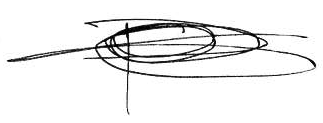
\includegraphics[width=5cm]{./img/signature.png}\\[.5cm]
\studenta
\end{center}

\emptypage

\chapter{\titel}
\label{ch:introduction}
\paragraph{The target audience.}
This thesis was written with an audience in mind that already has some technical understanding of computers and how they operate on hardware level (processor etc.). If you feel that your current knowledge is insufficient, or just want to read up some more, then I refer you to the ''How Computers Work - Processor and Main Memory'' \citep{Young2001} e-book.
\paragraph{The history of SPAM.} 
Ever since the internet found its way into our daily life, there have been people out there who don't always have other people's best interest in mind. I am referring to spammers, people aiming to advertise their product, services, etc \ldots in an aggressive manner. The methods of advertising include but are not limited to: \begin{itemize}
\item Sending bulk emails without the recipients permission (SPAM). 
\item Posting irrelevant links and information on fora and various social media.
\item Flooding chat channels with their links and information. 
\end{itemize}
These emails, posts and messages inconvenience the end-users, requiring time to filter out the junk. The economic costs of SPAM has led to a decrease in the Japanese GDP by 500 billion Yen (3.78 billion Euro) in 2004 and were projected to reach a decrease of 1\% of the total GDP by 2010 unless adequate countermeasures were taken \citep{Ukai2007}. \citep{Khong2004} researched the economic arguments for regulating junk mails and the efficiency of these regulations.
\paragraph{Birth of CAPTCHA.} 
The two previously mentioned researches signify the importance and impact of SPAM on our daily life. The users of the internet quickly tried to implement methods to prevent spammers from spreading their advertisements to the masses. Several prevention and detection methods and systems were developed successfully. These methods and mechanisms range from hidden text to invalid HTML tags, all used to confuse and interrupt automated programs. One of the methods developed to prevent SPAM is a CAPTCHA test. CAPTCHA is an acronym based on the word ''capture'' and stands for 'Completely Automated Public Turing test to tell Computers and Humans Apart'. An attempt to trademark  the term was made by Carnegie Mellon University on 15 October 2004, but the application was eventually dropped on 12 April 2008
\paragraph{Spammers fight back.}
All these prevention and detection methods did not stop the spammers from trying to reach an audience as large  as possible. The spammers rely on a large target audience because of the return rates being as low as 0.0023\% \citep{Cobb2003}. The spammers started to device ways to circumvent or break the existing systems in order to reach a large enough audience. One of these methods is solving CAPTCHA tests by making use of the adaptive learning and pattern recognizing capabilities of neural networks. These networks can be used to recognize letters from images with adversarial clutter.
This is the area I will focus on in this thesis. This thesis will list some of the difficulties regarding the extraction of relevant data from a CAPTCHA and how to possibly overcome these difficulties. However the main focus will be on understanding the inner workings of neural networks and on searching for the types and configuration of neural networks best used for pattern recognition.
\cleardoublepage
\chapter{Premise and research questions}
\label{ch:Premise}
\section{Premise}
\label{sec:Premise}
The main objective of this thesis is to ascertain whether neural networks are capable of solving the current generation of CAPTCHA images. we will define the premise  as following:\\\\
\emph{''Are neural networks a viable tool for solving the current generation of CAPTCHA?''}
\section{Research questions}
\label{sec:researquestions}
The research can be divided into two separate subjects. If one were to develop software for automatic CAPTCHA solving, the following questions and problems would need to be addressed.
\paragraph{\captcha :}
\begin{itemize}
\item What are CAPTCHAs?
\item Why were they developed?
\item Are there downsides to using CAPTCHA tests?
\end{itemize}
\paragraph{Neural networks:}
\begin{itemize}
\item How do neural networks operate?
\item Which types of neural networks are well suited for pattern recognition?
\item What network configuration would perform best?
\end{itemize}
\paragraph{General:}
\begin{itemize}
\item Will the solution be usable for long time?
\item Is there enough economic incentive to invest in development?
\end{itemize}
\cleardoublepage
\chapter{Methodology}
\label{ch:methodology}
This thesis is made up out of several parts, the first parts are a study on CAPTCHA and neural networks. The last part is a description of applying the gathered information.
\subsection{Research philosophy}
The research philosophy used in this thesis is post-positivism. It will use quantitative, qualitative and other methods (such as interpreting and combining several sources). The premise in this philosophy is that the world can be objectified, but the objectification is always coloured based on the subjective knowledge, experiences and beliefs of each individual.
\subsection{Approach}
Using a practical approach to the solving the CAPCTHA tests by implementing them in an experimental setting provided some obstacles. The information in this thesis was gathered primarily by performing literature studies on the subjects of these obstacles.
\cleardoublepage
\chapter{Corpus}
\label{ch:corpus}
\section{CAPTCHA}
\label{sec:captcha}
\subsection{CAPTCHA, an explanation}
A CAPTCHA (pronounced \textipa{/'k\ae p.\textteshlig \textschwa /}) is a type of challenge-response test that aims to make sure the response was made by a human. These tests are designed in such a manner that they should be easy to generate and grade by a computer, and at the same time be difficult for a computer to solve. while maintaining the rule that a human should be able to solve the test without much difficulty. If a test was solved successfully one can assume that the response was entered by a human.\\These test are mostly found on sites where one would like to prevent the access to unwanted bots\footnote{Automated scripts, in this context often used to gather personal information or used todistribute unwanted messages}. This is because having lots of spam on a site or in a service can have real detrimental consequences for that site or service. This is because most contemporary interactive sites store and serve their content from a database. When a database gets filled up the site can become slow and sluggish, degrading the customer's experience. This is only one of the many useful applications of CAPTCHAs. On the other hand, legitimate users also need to solve these tests, so it requires them to perform an extra task before they can post their content, create an email or view a certain page. While this 'simple' extra task does not seem like a large barrier, it does inconvenience some people enough to prevent them from posting valid content. This problem becomes even more apparent when dealing with non-native speakers \citep{Banday2011}. Protecting your site with a CAPTCHA can even have a detrimental effect on the conversion rates\footnote{\url{http://www.seomoz.org/blog/captchas-affect-on-conversion-rates}}.
\subsection{The history of CAPTCHA}
Moni Naor was the first one to think of the concept of CAPTCHA in 1996. He proposed that reverse Turing testing, as CAPTCHAs are often called, should consist of ''tasks where humans excel in performing, but machines have a hard-time competing with the performance of a three year old child.'' Some of these tasks were \citep{Naor1996}:
\begin{itemize}
\item gender recognition
\item understanding facial expressions
\item understanding handwriting
\item filling in words
\end{itemize}
In 1997 'Yahoo!' was having a gargantuan problem with spammers using bots to create free email addresses used to spread a huge amount of unwanted advertisement, giving Yahoo email adresses a bad reputation. 'Yahoo!' contacted Carnegie Mellon University\footnote{\url{http://www.cylab.cmu.edu/research/projects/2008/captcha-project.html}} for help, by 2000 the first real CAPTCHA as we know them was invented \citep{Egen2009}. These were also the people who first used the term ''CAPTCHA'' and tried to trademark it.\\As computing power increased, so did the amount of CAPTCHA tests being broken. By 2008 there was an 30\% to 60\% success rate on the most used CAPTCHA systems \citep{Yan2008}. As a  response to this Von Ahn and his team at Carnegie Mellon University released reCAPTCHA (Figure ~\ref{fig:reCAPTCHA}, page ~\pageref{fig:reCAPTCHA}) in September 2008, a popular system which is still in use.\\CAPTCHAs have always undergone changes once it became clear a certain generation method didn't stop the spammers anymore. The first CAPTCHAs generated by EZ-Gimpy for 'Yahoo!' looked completely different from the CAPTCHAs that are currently being generated. A good example of the adaptive nature of CAPTCHAs is reCAPTCHA, were you can see the changes depending on when a CAPTCHA was generated. (Figure ~\ref{fig:captchaEvolution}, page ~\pageref{fig:captchaEvolution})
\subsection{Types of CAPTCHA}
Following is a list and description of the different types of CAPTCHA, courtesy of \citep{Sauer2008}.
\begin{description}
\item[Character based]In this category a string of characters is presented to the user. This string can contain either words or random alphanumeric characters. The task is to identify the string of characters.
\item[Image based]In this category images or pictures are presented to the user. This is normally in the form of an identifiable real-world object, but can also be presented in the form of shapes. The task is to identify the object shown in the picture.
\item[Anomaly based]In this category a series of different objects, shapes, characters,\ldots is presented to the user. The task is to determine which object, character or shape does not belong in a set of images displayed on the screen.
\item[Recognition based]In this category all previous categories can be used. The user is tasked to determine what is being presented to them and respond accordingly.
\item[Sound based]In this category an audio version of a CAPTCHA is presented. The task is to identify the words and letters or image presented to the user.
\end{description}
\subsection{Data extraction}
As previously stated, the data extraction part of solving CAPTCHAs is not the main focus of this thesis. Therefore I will not give in-depth explanations of the algorithms used and described here.\\\\CAPTCHAs are by design tough to solve for a computer. The majority of times a CAPTCHA gets cluttered with noise, or the letters get crowed together. This crowding or noise makes it so that the characters on the image are not separate entities. This is to impede the segmentation of the CAPTCHA. Measures against segmentation are necessary to prevent an OCR\footnote{Optical Character Recognition} algorithm from simply reading and solving the test. This could be possible, as computers can (given the right algorithms) be very efficient at pattern recognition. People trying to solve the CAPTCHA test automatically, have to separate the individual characters first before they can pass the characters to an OCR algorithm for classification.\\\citep{Yan2008} described a working segmentation algorithm in 2008, but \citep{Huang2010} has significantly improved on the performance, so it should be able to segment the contemporary CAPTCHAs.\\In the unlikely case that the CAPTCHAs you are trying to solve don't have the segmentation issues, then you can first try to reduce the noise and then segment the characters by using the flood-fill method, as described by \citep{Cai2008}.
\subsection{The future of CAPTCHA}
The arms race between the makers of CAPTCHA systems and people trying to break them favoured the defender. This is different from other computer security arms races, where the odds are in favour of the adversary. This is because CAPTCHA has broken the traditional pattern where the attacker's role is to generate new instances while the defender must recognize them, recognizing a problem is almost always harder than generating them. Websites and services using CAPTCHA can easily change the CAPTCHA generation algorithm, creating new unsolvable CAPTCHAs, while the attackers now have the challenging recognition problem. This battle has brought advances to the field of Automated Pattern Recognition and Artificial Intelligence. Some people even believe that eventually the solving algorithms will become so sophisticated they could be classified as a sentient AI\footnote{\url{http://thenextweb.com/2009/10/15/inevitable-future-captcha/}} (Figure~\ref{fig:xkcdCAPTCHA}, page ~\pageref{fig:xkcdCAPTCHA}).\\
All the positive aspects and technological innovations aside, CAPTCHAs are inherently flawed. As the solving agents got better, the CAPTCHAs became harder. We have reached the point where the average user is having difficulties solving the standard CAPTCHAs\footnote{\url{http://www.internetevolution.com/author.asp?section_id=587&doc_id=259406}}. \\\\CAPTCHA of the future will need to explore completely new test systems. As an example of this, \citep{Sauer2008} and colleges did a small research about how the current CAPTCHA (even the audio CAPTCHA) has serious shortcomings when trying to accommodate for blind or visually impaired users. They suggest a new system were the sound and image part of the test are integrated, opposed to the current system where the audio part and the visual part are on independent development and maintenance paths. With their suggested test all visually impaired and hearing impaired users should be able to solve the test.\\\\
But even the newly developed systems will eventually succumb to the ever increasing computing power \citep{Beede2010}. The question is whether CAPTCHAs are the right way to prevent spammers, because how many ''unsolvable CAPTCHA'' (Figure ~\ref{fig:ImpossibleCaptcha}, page ~\pageref{fig:ImpossibleCaptcha}) is a user going to tolerate before giving up? The malcontent of some has even led to the creation of intentionally unsolvable CAPTCHAs (Figure ~\ref{fig:CRAPCHA}, page ~\pageref{fig:CRAPCHA}) through a service called ''CRAPCHA''\footnote{\url{http://crapcha.com/}}, aimed at ridiculing the real CAPTCHA services.
\begin{quote}
It would seem evident from years of use and research that CAPTCHAs are far from perfect as a solution. Remove spammers from the equation and we remove the need for CAPTCHAs entirely; this is the mentality we should be aiming for. The perfect CAPTCHA is no CAPTCHA at all. \citep{Bushell2011}
\end{quote}\newpage
\section{Neural Networks}
\label{sec:neuralnetworks}
The following section is a synthesis of 2 books describing neural networks, so similarities in structure and wording will be found. However, no malicious copyright infringement is intended. The two books used are ''Neural Networks'' by David Kriesel \citep{Kriesel2013} and ''Introduction to neural networks with Java'' by Jeff Heaton \citep{Heaton2005}.
\subsection{The concept of time}
When we describe time in the context of neural networks, we denominate the number of cycles of the neural network. In this context time is split into discrete steps.
\begin{definition}(The Concept of time). We reference the current time as $(t)$ the next step in time is referred to as $(t+1)$ and the previous step as $(t-1)$. The other steps further ahead or behind are referenced analogously. \end{definition} When we refer to a certain point in time for mathematical variables (e.g. $net_j or o_i$) we will do this as following $net_j(t-1) or o_i(t+3)$.
\subsection{The components of an artificial neural network}
An artificial neural network is made up by basic processing units, the \emph{neurons}, and directed weighted connections between these neurons. The strength of the connection is called the weight, this is expressed as $w_{i,j}$ for the connection between neuron $i$ and neuron $j$
\begin{definition}
(Neural network). A neural network is a sorted triple $(N, V, w)$ which contains two sets $N, V$ and a function $w$. $N$ is a set of neurons, $V$ is a set of connections where for each connections between neuron $i$ and $j$ applies $\{(i,j)|i,j \in  \mathbb{N}\}$, $w$ is a function ($w : V \to \mathbb{R}$) defining the weights. Where $w((i,j))$ defines the weight for the connection between neuron $i$ and neuron $j$, shortened to $w_{i,j}$.
\end{definition} Depending on the implementation, a connection in the network does not exist or has no influence when the weight is undefined or equal to zero. The weight can be combined in a square \emph{weight matrix} $W$, or in a \emph{weight vector} $W$. The row number indicates where a connection begins and the column number where it ends. In this representation, a zero indicates a non-existing or inactive connection. This kind of representation is also called a \emph{Hinton Diagram} (Figure ~\ref{fig:HintonDiagram}, page ~\pageref{fig:HintonDiagram}).
\subsubsection{Neuron Data Processing}
Upon closer inspection, we can see that the neuron and its connections are made up out of several other distinguishable components and processes. which we will discuss more in-depth in the following sections.
\begin{figure}
\centering
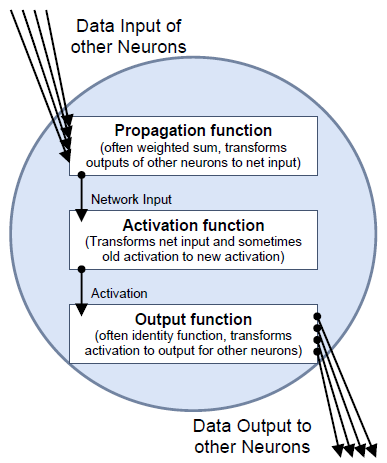
\includegraphics[width=7cm]{./img/Neuron_Dataprocessing.png}
\caption{Neuron Data processing (Source: \citep{Kriesel2013} page 39, Figure 3.1)}
\end{figure}
\subsubsection{Propagation function}
In a network there will likely be more then one neuron linking to neuron $j$. Which means that each neuron one of these neurons will pass its output to neuron $j$. The propagation function receives all these outputs $o_{i_{1}},\dotsc,o_{i_{n}}$ of the neurons $i_1,i_2,\dotsc,i_n$ and combines those into a single value, the \emph{network input} $net_j$, based on the connection weights $w_{i,j}$.
\begin{definition}
(Propagation function and network input) The network input, or $net_j$, can be calculated with the propagation function $f _{prop}$ as follows:
\begin{equation}
net_j = f _{prop}(o_{i_{1}},\dotsc,o_{i_{n}},w_{i_{1},j},w_{i_{n},j})
\end{equation}
Where $I = \{i_1,i_2,\dotsc,i_n\}$ is the set of neurons so that $\forall z \in \{1,\dotsc,n\} : \exists w_{i_{z},j}$. The \emph{weighted sum} is a very popular, and the most used propagation function.
\begin{equation}
net_j = \sum_{i \in I}(o_i \cdot w_{i,j})
\end{equation}
\end{definition}
\subsubsection{Neuron threshold value}
\begin{definition}
(Threshold value in general). The threshold value $\Theta_j$ for neuron $j$ is uniquely assigned to $j$ and defines the position of the maximum gradient of its activation function.
\end{definition}
This means that the activation function of a neuron will react very sensitive to changes when $net_j$ is around the threshold value. 
\subsubsection{Neuron activation function.}
\paragraph{Activation status.}Neurons can change in activation status. A neuron's activations state depends on the $net_j$, the previous activation state and the activation function. A neurons activation state is important, because this will influence a neuron's reaction to the $net_j$.
\paragraph{Activation function.}
\label{par:activationfunction}
The activation, also called the transfer function, $a_j$ of neuron $j$ depends on on previous states, so this will change overtime. The activation function uses the network input $net_j$, the threshold value and the previous activation state $a_j(t-1)$ to create a new \emph{activation state}. The neuron activation function is also called the identity.
\begin{definition}
(activation and activation function). In neuron $j$ the activation function can be described as
\begin{equation}
a_j(t) = f _{act}(net_j(t),a_j(t-1),\Theta_j)
\end{equation}
\end{definition}
\subparagraph{Binary threshold function.}
The binary threshold function, also called the \emph{Heaviside function}, is the simplest activation function as can only take on two values. The activation will change, depending on whether the input value is above or below the threshold value. In either case the function changes from one value to another. This activation function doesn't have a variable, hence it's derivative is 0. This makes back-propagation learning impossible 
\subparagraph{Fermi function.}
The Fermi function, also called the logistic function, uses following equation. from the equation we can derive that the Fermi function maps a range of values between $(0,1)$. It's function is describe as following:
\begin{equation}
\displaystyle \frac{1}{1+e^{-x}}
\end{equation}
\subparagraph{hyperbolic tangent.}
The hyperbolic tangent function maps to values within the range of $(-1,-)$. It's function is describe as following:
\begin{equation}
\tan(x)
\end{equation}
\subparagraph{Fermi function with temperature parameter.}
The Fermi function can be expanded by adding a temperature parameter. The smaller this parameter becomes the colder the activation function becomes, the steeper the gradient of the activation function becomes. And visa versa. By making the temperature parameter very small, we can emulate the Heaviside activation function's behaviour. The extended Fermi activation is described as following:
\begin{equation}
\displaystyle \frac{1}{1+e^{\frac{-x}{T}}}
\end{equation}
\subsubsection{The bias neuron}
\label{subsubsec:biasneuron}
The bias neuron (also called the on neuron) is a technical trick. The purpose of a bias neuron is to represent a neurons threshold value as a connection weight. As said before the activation of a neuron depends on its threshold value, however theses threshold values are stored inside the neuron itself. This makes it complicated to access and use in the activation function, or to train the threshold value. This is where the bias neuron comes in.\\\\Threshold values $\Theta_{j_{i}}, \dotsc ,\Theta_{j_{n}}$ for neurons $j_1,j_2, \dotsc ,j_n$ can be expressed as a connection weight of a constantly firing neuron. This constantly firing neuron is the bias neuron. To implement this change, an additional neuron, whose output is always 1, will be added tot the network and connected to neurons $j_1,j_2, \dotsc ,j_n$. The newly made connections' weights will be set to the negative threshold values. $w_{BIAS,j_{n}} = - \Theta_{j_{n}}$\\\\Now that the threshold values are implemented as connection weight, the threshold value $\Theta_{j_{n}}$ of neurons $j_1,j_2, \dotsc ,j_n$ is then set to 0. This also means that the threshold value can be directly trained together with the connection weight. This makes the learning process considerably easier. Since the threshold value is no longer included in the activation function, its effect is now included in the propagation function.\\\\The advantages of the bias neuron are obvious when implementing and training a neural network. However they do have a disadvantage when you want to visually represent the neural network. These extra connection quickly clutter up the visual representation, and this becomes only worse when a lot of neurons are being used. But since the implementation of a bias neuron is almost a certainty, a lot of people omit the bias neuron from their illustrations for improved clarity. We know it exist and know that threshold values can simply be treated as weights because of it.
\begin{definition}
(Bias neuron). A bias neuron is a neuron whose output value is always 1 and is used to represent neuron biases as connection weights, which enables any weight training algorithm to train the biases at the same time.\\\\Let $j_1,j_2, \dotsc ,j_n$ be neurons with threshold values $\Theta_{j_{1}}, \dotsc ,\Theta_{j_{n}}$. By inserting a bias neuron whose output value is always 1, generating connections between the bias neuron and neurons $j_1,j_2, \dotsc ,j_n$ and weighting these connections $w_{BIAS,j_{1}},\dotsc,w_{BIAS,j_{n}}$ with $\Theta_{j_{1}}, \dotsc ,\Theta_{j_{n}}$, we can set $\Theta_{j_{1}}= \ldots = \Theta_{j_{n}} = 0$ and receive an equivalent neural network whose threshold values are realized by connection weights.
\end{definition}
\subsubsection{Neuron activation order.}
The sequence in which the neurons of a neural network receive and process the input is critical for the result.
\paragraph{Synchronous activation.}
In this activation scheme all neurons update at the same time. They simultaneously calculate the input, activation and output. This type of activation scheme closest resembles biological neural networks. However implementing this is only possible on hardware capable of parallel processing. This is the most generic activation scheme and can be used for any network, independent of network topology. However feedforward networks would not benefit from this scheme.
\paragraph{Asynchronous activation.}
The counterpart of synchronous activation. The neurons won't fire all at once in this scheme, but in different points in time. Several subcategories can be discerned. 
\subparagraph{Random order activation.}
In this activation scheme, a random neuron $i$ is chosen from all the neurons and for that neuron the input. For an $n$ neuron network, the activation cycle will end after having update $n$ neurons. During this random cycle some neurons can be update multiple times, while others don't get updated at all. It is for this reason that this order of activation is not always useful.
\subparagraph{Random permutation activation.}
In this scheme a list of each neuron in a randomized order is made. Therefore during one cycle, each neuron will be activated exactly once. But in a random order.\\
This activation order doesn't get used much, just like random order activation. This is because of the huge overhead generated by having to build a random order list of each neuron for each activation cycle. While Hopfield network topology technically should be updated at random, in practice a fixed order activation is preferred.
\subparagraph{Topological order activation.}
In this scheme the neurons are update in a fixed order. The order is defined by the network topology. First the input neurons get activated then the layer after that, and so on until the output neurons are reached. Due to the definition, this activation order cannot be used for recurrent networks as they don't have a clearly defined start or end. This is the most efficient activation schema when comes to feedforward networks.
\subparagraph{Fixed order activation.}
In this scheme the order of activation gets set during implementation. This can be useful in some cases (again feedforward networks come to mind), but in case a network can change topology during runtime, then this activation order will have detrimental effects, because it cannot and will not change based on the new topology.
\subsubsection{Neural output function}
The output function calculates what value neuron $i$ will pass to its connected neurons $j$. The output value $o_j$  of neuron $j$ is calculated from its activation state $a_j$.
\begin{definition}
(Output function). For neuron $j$ the output function is formally described as
\begin{equation}
f _{out}(a_j) = o_j
\end{equation}
Generally though the output functions is often the same as the activation $a_j$, which is directly output.
\begin{equation}
f _{out}(a_j) = a_j,SO o_j = a_j
\end{equation}
\end{definition}
\subsubsection{Input and output of data}
The purpose of a neural network is to receive, process and return data. The input components for a network with $n$ input neurons can be scribed by vector $x = (x_1,x_2, \dotsc ,x_n)$ and the output components for a network with $m$ output neurons can be scribed by vector $y = (y_1,y_2, \dotsc ,y_m)$. this leads us to following definitions:
\begin{definition}
(Input vector). A network with $n$ input neurons needs $n$ input values $x_1,x_2, \dotsc ,x_n$ they can be combined in an input vector $x = (x_1,x_2, \dotsc ,x_n)$.
\end{definition}
\begin{definition}
(Output vector).  A network with $m$ output neurons has $m$ output values $y_1,y_2, \dotsc ,y_m$ they can be combined in an input vector $y = (y_1,y_2, \dotsc ,y_m)$.
\end{definition}
\subsection{Neural network topologies}
Until now, we have only looked at the different elements that make up a neuron. But we can only do so much with only one neuron. It is time to zoom out and start looking at how several neurons can be organized together to effectively make a neural network. The following is a list of the usual network designs. Every topology described will be accompanied by a visual representation a Hinton diagram, courtesy of \citep{Kriesel2013}. The Hinton diagram is supplied so that the characteristics of the network can immediately be seen.\\\\For the transformation from the visual representation tot the Hinton diagram, following legend will be used:
\begin{itemize}
\item dotted weight connections will be represented as light gray fields
\item solid weight connections will be represented as dark grey fields
\item the directional arrows cannot be added. So to express that connections start from the line neurons and end at the column neurons, the $\Rsh$ symbol has been introduced in the upper left corner.
\end{itemize}
\subsubsection{Feedforward networks}
\paragraph{Standard feedforward network.\label{par:feedforward}} The first topology we will discuss is the one of the standard feedforward network. In a feedforward network the neurons are divided into layers. These layers can be grouped in three types of layers: one \emph{input layer}, $n$ \emph{hidden layers} and one \emph{output layer}. The hidden layers cannot be seen from the outside (hence the name hidden), and the neurons in those layers are referred to as hidden neurons. The hidden layers are also often referred to as the processing layers. In a feedforward network, a neuron has only connections towards the next layer. These connections all are directed towards the output layer. In many cases we will find that each neuron $i$ is connected to every neuron $j$ of the next layer. These networks are called completely linked feedforward networks. As a naming convention, the output neurons will often be referred to as $\Omega$. (Figure ~\ref{fig:feedforward})
\begin{definition}
(Feedforward network). 
\end{definition} A feedforward network consists of three types of layers, one input layer, one output layer and optionally one or more processing layers. These layers are clearly separated. Connections only go from one neuron layer to the next, directed towards the output layer.
\begin{figure}
\centering
	\begin{subfigure}[b]{0.49\textwidth}
	\centering
	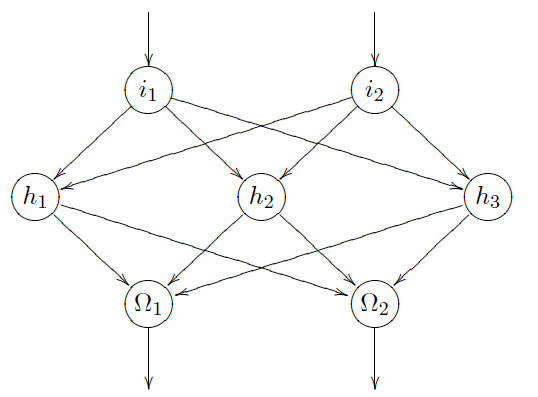
\includegraphics[width=\textwidth]{./img/Feedforward-normal-Topology.png}
	\caption{Standard feedforward topology}
	\end{subfigure}
	\begin{subfigure}[b]{0.49\textwidth}
	\centering
	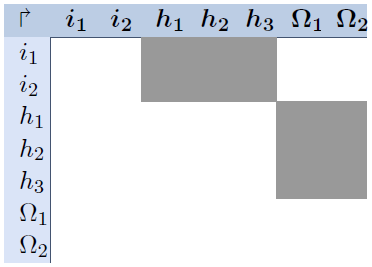
\includegraphics[width=\textwidth]{./img/Feedforward-normal-Hinton.png}
	\caption{Standard feedforward Hinton diagram}
	\end{subfigure}
\caption{Standard feedforward network; Source:\citep{Kriesel2013}}
\label{fig:feedforward}
\end{figure}
\paragraph{Shortcut connections.}
This is essentially a standard feedforward network (see ~\ref{par:feedforward}) where connections exist that skip one or more levels. These so-called shortcut connections may only be directed towards the output layer. (Figure ~\ref{fig:shortcutfeedforward})
\begin{definition}
(Shortcut feedforward). A shortcut feedforward network consists of three types of layers, one input layer, one output layer and optionally one or more processing layers. These layers are clearly separated. Connections only exist directed towards the output layer, the connections however may span over one or more layers.
\end{definition}
\begin{figure}
\centering
	\begin{subfigure}[b]{0.49\textwidth}
	\centering
	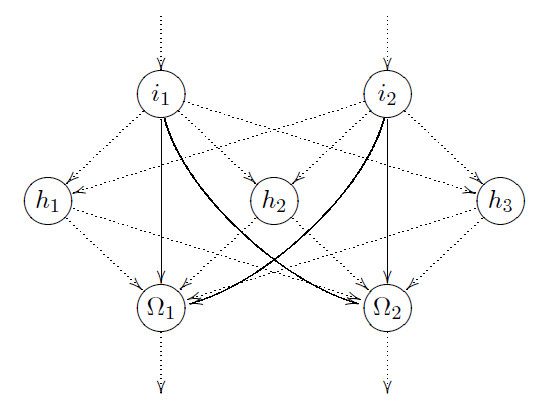
\includegraphics[width=\textwidth]{./img/Feedforward-shortcut-Topology.png}
	\caption{Shortcut feedforward topology}
	\end{subfigure}
	\begin{subfigure}[b]{0.49\textwidth}
	\centering
	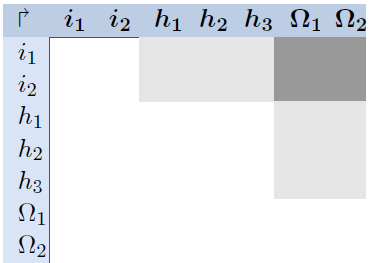
\includegraphics[width=\textwidth]{./img/Feedforward-shortcut-Hinton.png}
	\caption{Shortcut feedforward Hinton diagram}
	\end{subfigure}
\caption{Shortcut feedforward network; Source:\citep{Kriesel2013}}
\label{fig:shortcutfeedforward}
\end{figure}
\subsubsection{Recurrent networks}
Recurrence is the event where a neuron influences itself. This can be done through any means or by any connection. It is because of this that recurrent networks often don't have explicitly defined input and output neurons.
\paragraph{Direct recurrent.}
Direct recurrence happens in a network when neurons feed their output back to themselves as input. This is also often called self-recurrence. The neurons inhibit themselves, and as a result of this strengthen themselves in order to reach their activation limits. (Figure ~\ref{fig:directrecurrent})
\begin{definition}
(Direct recurrence). A direct recurrence network is a network where a neuron $j$ is connected to itself. The connection weight is then defined as $w_{j,j}$. The diagonal of weight matrix $W$ will no longer be zero as a direct result from this.
\end{definition}
\begin{figure}
\centering
	\begin{subfigure}[b]{0.49\textwidth}
	\centering
	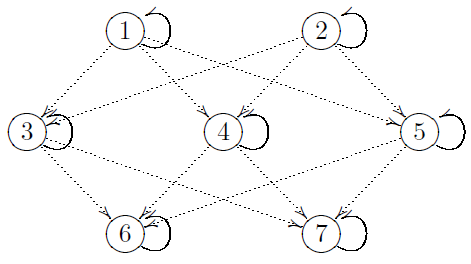
\includegraphics[width=\textwidth]{./img/recurrent-direct-Topology.png}
	\caption{Direct recurrent topology}
	\end{subfigure}
	\begin{subfigure}[b]{0.49\textwidth}
	\centering
	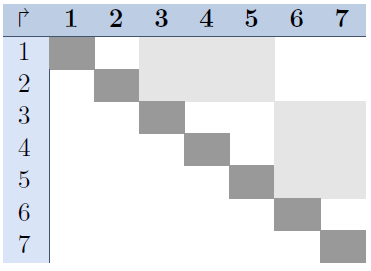
\includegraphics[width=\textwidth]{./img/recurrent-direct-Hinton.png}
	\caption{Direct recurrent Hinton diagram; Source:\citep{Kriesel2013}}
	\end{subfigure}
\caption{Direct recurrent network}
\label{fig:directrecurrent}
\end{figure}
\paragraph{Indirect recurrent.}
Indirect recurrence happens when in a network connections towards the input layer are allowed. A neuron can influence itself by passing its output to one of the previous or one of the next layers. (Figure ~\ref{fig:inderectrecurrence})
\begin{definition}
(Indirect recurrence). An indirect recurrent network is a network where connections forward and backward in the network may exist. The neurons influence themselves by influencing the preceding layers.
\end{definition}
\begin{figure}
\centering
	\begin{subfigure}[b]{0.49\textwidth}
	\centering
	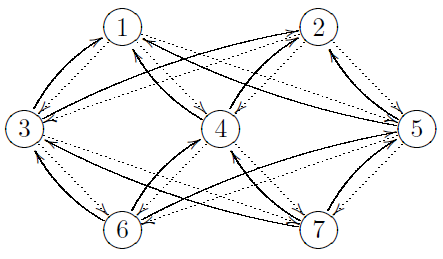
\includegraphics[width=\textwidth]{./img/recurrent-indirect-Topology.png}
	\caption{Indirect recurrent topology}
	\end{subfigure}
	\begin{subfigure}[b]{0.49\textwidth}
	\centering
	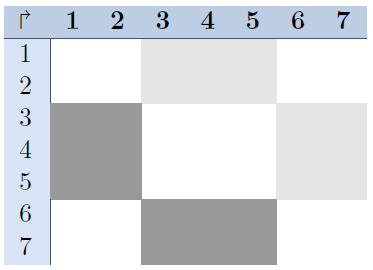
\includegraphics[width=\textwidth]{./img/recurrent-indirect-Hinton.png}
	\caption{Indirect recurrent Hinton diagram; Source:\citep{Kriesel2013}}
	\end{subfigure}
\caption{Indirect recurrent network}
\label{fig:inderectrecurrence}
\end{figure}
\paragraph{Lateral recurrent.}
Lateral recurrence happens when connections between neurons of the same layer exist. These connections often make it so that each neuron inhibits the other neurons and strengthens itself. This often means that only the strongest neuron becomes active (\emph{winner-takes-all scheme}). (Figure ~\ref{fig:lateralrecurrence})
\begin{definition}
(Lateral recurrence). A lateral recurrent network is a network where connections between the neurons of the same layer are allowed.
\end{definition}
\begin{figure}
\centering
	\begin{subfigure}[b]{0.49\textwidth}
	\centering
	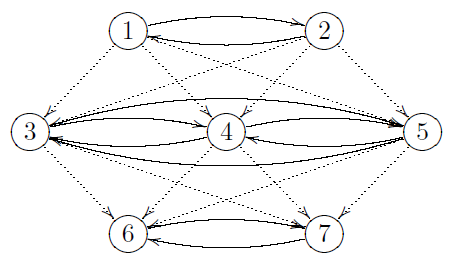
\includegraphics[width=\textwidth]{./img/recurrent-lateral-Topology.png}
	\caption{Lateral recurrent topology}
	\end{subfigure}
	\begin{subfigure}[b]{0.49\textwidth}
	\centering
	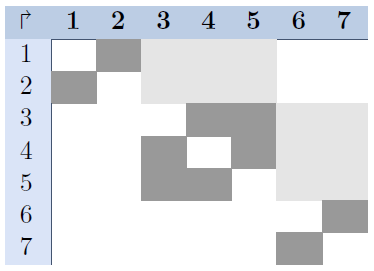
\includegraphics[width=\textwidth]{./img/recurrent-lateral-Hinton.png}
	\caption{Lateral recurrent Hinton diagram; Source:\citep{Kriesel2013}}
	\end{subfigure}
\caption{Lateral recurrent network}
\label{fig:lateralrecurrence}
\end{figure}
\subsubsection{Completely linked networks}
A completely linked network happens when all neuron connections are allowed, except for direct recurrent connections. All neuron connections must be symmetric, this means that $w_{i,j} = w_{j,i}$. As a direct result of the complete linking, input and output neurons can no longer be strictly defined and clearly defined layers do not longer exist. Another result is that the weight matrix $W$ can be different from zero everywhere, except along the diagonal. (Figure ~\ref{fig:completelylinked})
\begin{definition}
(Complete interconnection). A complete interconnected network is a network where each neuron is always connected to every other neuron. As a result every neuron can become an input neuron.
\end{definition}
\begin{figure}
\centering
	\begin{subfigure}[b]{0.49\textwidth}
	\centering
	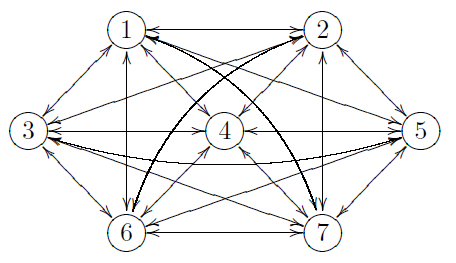
\includegraphics[width=\textwidth]{./img/Completelylinked-Topology.png}
	\caption{Completely linked topology}
	\end{subfigure}
	\begin{subfigure}[b]{0.49\textwidth}
	\centering
	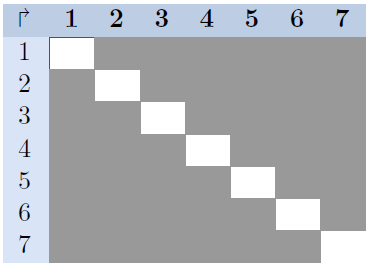
\includegraphics[width=\textwidth]{./img/Completelylinked-Hinton.png}
	\caption{Completely linked Hinton diagram; Source:\citep{Kriesel2013}}
	\end{subfigure}
\caption{Completely linked network}
\label{fig:completelylinked}
\end{figure}
\subsection{Neural network learning}
One of the most interesting features of a neural network is the ability to familiarize themselves with a problem by means of training. This means that after sufficient training, the network will be able to solve unknown problems of the same type. This is called generalization. Training a  network involves some form of learning procedure. A learning procedure is a rather complex thing, so a brief explanation will be given first.
\paragraph{Learning paradigms.}
We must be careful with the term ''learning'' as it is a very comprehensive term. A system learns when it changes itself in order to adapt to changes in the systems environment. A neural network as a learning systems changes, learns, whenever its components change. So any change in the components previously  mentioned due to environmental changes will result in a changing network. This process is classified as neural network learning. Looking ad the previous components capable of changing we can form a list of all theoretically possible means of neural network learning.
\begin{enumerate}
\item developing new connections
\item deleting existing connections
\item changing connecting weights
\item changing the threshold values of neurons
\item varying one or more of the three neuron functions (activation function, propagation function and output function)
\item developing new neurons
\item deleting existing neurons (and so its existing connections)
\end{enumerate}
We can safely assume that changing the connection weights will be the most commonly used method of training. Especially because of the simple fact that deleting a connection (no longer training a connection with weight) and creating new connections (changing the connection weight from 0) in the connection matrix can be done by connection weight adjustment training. With the introduction of the bias neuron (~\ref{subsubsec:biasneuron}) the threshold values can also be changed by using connection weight training.  We can perform any of the first four of the learning paradigms by just training synaptic weights.\\\\Changing neuron functions is difficult to implement and not very intuitive. Because of this, those paradigms aren't really popular and will not be discussed any further. The option of generating new, or removing old neurons have a few advantages. This method not only provides a way to keep the connection weights well adjusted during the training of a neural network, it also optimizes the neural network topology. For this reason this type of training is gathering a growing amount of interest. A method of achieving this functionality would be evolutionary algorithms. However we will not elaborate any further on this since this is outside the scope of this thesis, and since we already covered that the majority of learning methods can be achieved by weight training.\\\\To summarize, neural network learn by modifying the connecting weights according to rules formulated as algorithms. Therefore a learning procedure is always an algorithm that can easily be implemented by means of a programming language.
\paragraph{Training patterns, teaching input, desired output and error vector}
\begin{definition}
(Desired output). The expected result of the output layer when presented with a training pattern.
\end{definition}
\begin{definition}
(Teaching input). For an output neuron $j$ the teaching input $t_j$ is desired and correct value $j$ should have after the input of a training pattern. The teaching inputs $t_1,t_2, \dotsc ,t_n$ van be combined into a vector $t$. $t$ always refers to a specific training pattern $p$. this correlation is contained in the training set.
\end{definition}
\begin{definition}
(Training pattern). A training pattern is an input vector $p$ with the components $p_1,p_2, \dotsc , p_n$ whose desired output is known. By entering the training pattern into the network we receive an output that can be compared with the desired output. 
\end{definition}
\begin{definition}
(Training set). A training set (named $P$) is a finite set of pairs of training patterns ($p$) and teaching inputs ($t$). The finite ordered pairs $(p,t)$ of training patterns and teaching inputs are used to train our neural network.
\end{definition}
\begin{definition}
(Error vector).The error vector (also called the difference vector) for output neurons $\Omega_1,\Omega_2, \dotsc ,\Omega_n$ is the difference between the actual output vector and the teaching input for a training input $p$. Depending on whether you are learning offline or online, the difference vector refers to a specific training pattern, or to the error of a set of training patterns which is normalized in a certain way.\begin{center}
$E_p = 	\begin{pmatrix}
			t_1-y_1\\
			t_2-y_2\\
			\vdots\\
			t_n-y_n
		\end{pmatrix}$
\end{center}
\end{definition}
\subparagraph{Unsupervised learning.}
Unsupervised learning is the type of learning closest related to how biological neural networks operate, yet this type of learning is not suitable for all problems. In this learning type only the training patterns are given, the network itself is taxed with trying to identify and classify similar patterns.
\begin{definition}(Unsupervised learning). The training set only consists of input
patterns, the network tries by itself to detect similarities and to generate pattern
classes.
\end{definition}
\subparagraph{Reinforcement learning.}
Reinforcement learning uses only the training patterns, but after each cycle a logical or real value is returned to it. This value indicates whether the output was correct or not.
\begin{definition}
(Reinforcement learning). The training set consists of input patterns,
after completion of a sequence a value is returned to the network indicating whether
the result was right or wrong and, possibly, how right or wrong it was.
\end{definition}
\subparagraph{Supervised learning.}
Supervised learning uses a training set $P$ consisting of both the trainings pattern $(p)$ and teaching input $(t)$ in form of the precise activation of all output neurons $\Omega$. The network is fed with the trainings patterns, and the connection weights then are adjusted based on the error vector obtained from subtracting the actual output with the teaching input. The goal is to change the weights in such a matter that the network cannot only associate input and output patterns independently after the training, but that is can also provide plausible results to unknown, similar input patterns. After training the network should be able to generalise.
\begin{definition}
(Supervised learning). The training set consists of training patterns and teaching inputs so that the network can calculate a precise error vector to adjust the network with.
\end{definition}
\subparagraph{Offline learning or online learning.}
Offline learning is a method that stands in stark contrast with online learning.\\In offline learning you present all training patterns at once and the total error is calculated with an error function, or simply accumulated. Only after all patterns have been presented will the weights be changed. Offline training procedures are also called batch training procedures, since a batch of results is corrected in one go. Such an iteration of a batch training process is called  epoch.\\In online learning the weights are changed after every pattern presented.\\\\Each method has advantages and disadvantages, and it isn't always clear what type is best to be used. 
\begin{definition}
(Offline learning). Several training patterns are entered into the
network at once, the errors are accumulated and it learns for all patterns at the same
time.
\end{definition}
\begin{definition}
(Online learning). The network learns directly from the errors of each
training sample.
\end{definition}
\paragraph{Training samples}
We should take a look at selecting the training data and the learning curve now that we know how to train a network. We should be particularly interested in whether our network has merely memorized the our training data (can it produce the right output for our trained inputs but to provide wrong answers for all other problems of the same class), or whether it can generalize the problem.\\\\It can be that the network has sufficient storage capacity to store the training data, but only recognizes the input data. This implies that the network is oversized and has to much free storage capacity. On the other it can be that the network has insufficient storage capacity, this in turn leads to bad generalization. It is important to find a balance.\\\\It is for this purpose that the trainingset is often divided into a set used for training the network, and a set used for verification. Provided of course that there are enough training samples not to affect the initial quality of training. The usual used ration is 70\% for training data and 30\% for verification. These sets should be randomly chosen. We can conclude the training of the network when both the results of the training data and the verification data are good. The verification data is included in the training, even though it is not directly used in training the network. What this means is that you do not modify the network to accommodate for the poor results of the verification data. If you do this, you run the risk of tailoring the network to the verification data. A  possible solution is a third set of validation data used only for validation after a supposable successful training. The downside to keep in mind is that by training less patterns, we obviously withhold information from the network and risk to worsen the learning performance.
\paragraph{Learning curve and error measurement}
A learning curve indicates the variations in the error. The motivation for creating a learning curve is to see whether the network is progressing or not. The error must first be normalized before we can use it to plot out the learning curve. Normalizing the error is to represent the distance between the correct and current output of the network. There are four ways of calculating the normalized error. In the following sections $\Omega$ will be the output neurons and $O$ the set of output neurons.
\subparagraph{Specific error.}
The specific error $Err_p$ is based on single training sample $p$. This means it is generated during online learning.
\begin{equation}
Err_p = \frac{1}{2} \sum_{\Omega \in O}(t_\Omega - y_\Omega)^2
\end{equation}
\subparagraph{Root mean square.}
The root mean square (also referred to as RMS) of two vectors $t$ and $y$ is a error normalization method that can be used both for online and offline.\\\\
The online formula:
\begin{equation}
Err_p =  \sqrt{\frac{\sum_{\Omega \in O}(t_\Omega - y_\Omega)^2}{|O|}}
\end{equation}
The offline formula:
\begin{equation}
Err = \sum_{_{p} \in P}\sqrt{\frac{\sum_{\Omega \in O}(t_\Omega - y_\Omega)^2}{|O|}}
\end{equation}
\subparagraph{Euclidean distance.}
Just like the root mean square the Euclidean distance calculates the error based on the two vectors $t$ and $y$, and can be used both online and offline.\\\\
The online formula:
\begin{equation}
Err_p =  \sqrt{{\sum_{\Omega \in O}(t_\Omega - y_\Omega)^2}}
\end{equation}
The offline formula:
\begin{equation}
Err = \sum_{_{p} \in P}\sqrt{{\sum_{\Omega \in O}(t_\Omega - y_\Omega)^2}}
\end{equation}
This is just a small grasp out of the most used error measuring methods, many more can be used. I you are interested in finding out more about error measurement please read the technical report of Prechelt \citep{Prechelt1994}\\\\Depending on the method used our learning curve will look different. Normally a perfect learning curve will look like a negative exponential function. A learning curve will be proportional to $e^{-t}$ so it can best be represented on a logarithmic scale. In this scale a descending line indicates an exponential decrease of the error.
\subparagraph{When to stop learning?}
Generally learning is stopped when the user ''thinks'' the error became small enough. There is no clear-cut answer for this question, but the analysis and comparison of learning curves can bring more clarity. You can also assume greater confidence, when a network reaches nearly the same final error-rate for different random initializations.\\\\A learning curve descending fast can be overtaken by another curve. This can indicate that either the learning rate of the worse curve was too high or the worse curve itself simply got stuck in a local minimum, but was the first to find it. It is also important to plot the verification data on a second learning curve. This will often provide worse result, but with good generalization this curve can decrease too.\\\\Preventing memorization of the sample data can be achieved by early stopping. An indication that early stopping might be beneficial is when the learning curve of the verification samples suddenly rises rapidly while the learning curve of the verification data is continuously falling
\paragraph{Hebbian rule}
The Hebbian learning rule acts as basis for most other complex learning rules. It was first described by \emph{Donnald O. Hebb} \citep{Hebb1949} and currently exists in 2 forms, the original rule and the generalized form.
\subparagraph{The original rule.}
\begin{definition}
(Hebbian rule). If neuron $j$ receives an input from neuron $i$ and if both neurons are strongly active at the same time, then increase the weight $w_{i,j}$, strengthening the connection.
\begin{equation}
\Delta w_{i,j} \sim \eta o_ia_j
\end{equation}
\end{definition}
With $\Delta w_{i,j}$ being the change in weight from $i$ to $j$. This change in weight is simply added to the weight $w_{i,j}$. $\Delta w_{i,j}$ is dependent on following factors.
\begin{itemize}
\item the output $o_i$ of predecessor neuron $i$
\item the activation function of successor neuron $j$
\item the constant $\eta$, the learning rate
\end{itemize}
Notice that the definitions speaks about the activation twice, while in the formula the activation is only used once. Instead of the activation $a_i$ of neuron $i$ and the activation$a_j$ of neuron $j$, the formula uses the activation $a_j$ of neuron $j$ and the output $o_j$ of neuron $i$. This is possible because the identity or activation of a neuron is often used as the output (~\ref{par:activationfunction}). Therefore $a_i$ and $o_i$ can be considerate as being the same value.
\subparagraph{Generalized form.}
\begin{definition}
(Hebbian rule, generalized). The generalized form of the Hebbian Rule only specifies the proportion of change in the weight based on the product of two undefined functions, but with defined input values.
\begin{equation}
\Delta w_{i,j} = \eta \cdot (h(o_i,w_{i,j}) \cdot g(a_j,t_j))
\end{equation}
\end{definition}
\label{equa:generalizedHebbian}
With $\Delta w_{i,j}$ being the change in weight from $i$ to $j$. This change in weight is simply added to the weight $w_{i,j}$. $\Delta w_{i,j}$ is dependent on following factors.
\begin{itemize}
\item $g(a_j,t_j)$: this function uses the actual activation $a_j$ and the expected activation found in the teaching input $t_j$
\item $h(o_i,w_{i,j})$: this function uses the output of the predecessor neuron $o_i$ and the connection weight between the two neurons $w_{i,j}$
\item the constant $\eta$, the learning rate
\end{itemize}
Since this is a generalized form, the functions $g$ and $h$ are not specified.
\paragraph{The learning rate.}
The speed and accuracy of a learning procedure are be controlled by and are always proportional to a learning rate $(\eta)$. If this value is chosen too big, it is possible to miss possibly favourable narrow local minima in the error. However, setting it very small is not a good solution either as this would dramatically increase the time and computing cost of training a network. Experience has shown that learning rates between 0.01 and 0.9 are mostly optimal. A popular method for finding an optimal $\eta$ is starting out high and slowly decreasing it.
\begin{definition}
(Learning rate). The learning rate $(\eta)$ dictates the speed and accuracy of a learning procedure.
\end{definition}
\section{Neural networks for pattern recognition}
We will take a look at several neural network implementations now that we have a clear understanding of how neural networks work and can be trained, . This thesis will focus on the network implementations most frequently found in the literature to be used for pattern recognition.
\subsection{Perceptron networks}
This is the classic example of neural network, often when the term ''neural network'' is used a perceptron network (or variation thereof) is meant. Perceptron networks were first described by Frank Rosenblatt in 1958 \citep{Rosenblat1958}. \\\\There is no set definition of a perceptron network, but it is often described as being a feedforward network with shortcut connections. The input layer of the the perceptron network is called the retina, and is only used for data input. No processing happens in the input layer as the weights for the input layer are static.
\subsubsection{Single layer perceptron network}
A single layer perceptron (or SLP for short) is a perceptron network that has only one layer (except the input neurons). This means that the trainable connection weights going from the input layer go straight towards one or more output neurons $\Omega$. A single layer perceptrons with multiple outputs can simply be considered as several separate single layer perceptrons with the same input. The single layer perceptrons is because of the limitation to a single layer only able to represent linear data.
\paragraph{Single layer perceptrons and the delta rule.}
The delta rule is an extension on the Hebbian rule. It has the advantage that it can be used with networks without binary activation functions, and that the network will automatically learn faster when it is farther away from the target. I refer you to the book ''Neural networks'' page 90-95 \citep{Kriesel2013} in case you want to read the whole mathematical and logical construction of the delta rule.
\begin{definition}
(Delta rule). The delta rule (also called the Widrow-Hoff rule) is based on the generalized Hebbian rule (~\ref{equa:generalizedHebbian}), where the function $h$ only uses the output $o_i$ of the predecessor neuron $i$, and where the function $g$ is the difference between the desired activation $t_\Omega$ and the actual activation $a_\Omega$ of the output neuron $\Omega$. If we substitute this into the Hebbian rule we get he following:
\begin{equation}
\Delta w_{i,\Omega} = \eta \cdot o_i \cdot (t_\Omega - a_\Omega) = \eta o_i \delta_\Omega
\end{equation}
\label{equa:deltaSLP}
If we were to use the desired output instead of the desired activation the formula would look like this:
\begin{equation}
\Delta w_{i,\Omega} = \eta \cdot o_i \cdot (t_\Omega - o_\Omega) = \eta o_i \delta_\Omega
\end{equation}
\end{definition}
These formulas can be used for online learning, in the case of batch processing you simply let the error accumulate
\begin{equation}
\Delta w_{i,\Omega} = \eta \cdot \sum_{_{p} \ in P} o_{p,i} \cdot (t_{p,\Omega} - o_{p,\Omega}) = \eta \cdot \sum_{_{p} \ in P} o_{p,i} \cdot \delta_{p,\Omega}
\end{equation}
\subsubsection{Multilayer perceptron network}
The multilayer perceptron (MLP for short) can represent functions with a higher than linear dimension, contrary to single layer perceptron. This achieved by taking a single layered perceptron with multiple output neurons and attaching other single layer perceptrons to this, to further process the already linear processed output from the output neurons of the base single layer perceptron. Each added layer supposedly adds the capability to process an extra dimension.\\\\It has been mathematically proven that even a multilayer perceptron with only one layer of hidden neurons can approximate a functions with finitely many discontinuities as well as their first derivatives to an arbitrary precision. This proof can unfortunately not be used in the reverse way, so it still is up to us to find the correct amount of neurons to use in each situation.\\\\When describing a multilayer perceptron comprising 7 input neurons, a hidden layer of 10 neurons, another hidden layer of 5 neurons and an output layer of 6 neurons the following abbreviation is often used: 7-10-5-6.\\The numbers indicate the amount of neurons for that layer. The first layer is the input layer (retina) and the last is the output layer. The layers in between are the hidden layers, these are always order going from closest to the input layer (and farthest from the output) to farthest from the input layer (and closest to the output).\\\\Word of warning for reading through the literature. Not all sources use the same way of counting the network layers, some include the retina, some count the trainable weight layers and others exclude the output neuron layer.
\paragraph{Multilayer perceptrons backpropagation.}
The backpropagation of error learning rule is used to train multi-staged neural perceptrons. Backpropagation is a gradient descent procedure with error function $Err(W)$ receiving all the connection weights as arguments and links them to the output error. This system is an extension of the delta rule. The output function is kept the same for each neuron, but the variable $\delta_i$ for each neuron $i$ needs to be generalized from one trainable weight to several ones. Again, if you want to read the whole mathematical and logical construction, please read \citep{Kriesel2013} pages 104-108.
\begin{definition}
(Backpropagation). Backpropagation is based on the generalized Hebbian rule (~\ref{equa:generalizedHebbian}), where the function $h$ only uses the output $o_i$ of the predecessor neuron $i$, and where the function $g$ is the difference between the desired activation $t_\Omega$ and the actual activation $a_\Omega$ of the output neuron $\Omega$. If we substitute this into the Hebbian rule we get the following:
\begin{equation}
\begin{array}{l l}
\Delta w_{i,j} : \eta \cdot o_i \cdot \delta_j \text{with}\\
\delta_j = \left\{
	\begin{array}{l l}
    f'_{act}(net_j) \cdot (t_j - y_j) & \quad \text{(when $j$ is an output neuron)}\\
    f'_{act}(net_j) \cdot \sum_{l \in L}(\delta_lw_{h,l})) & \quad \text{(when $j$ is a hidden neuron)}
  \end{array} \right.
\end{array}
\end{equation}
\end{definition}
\subparagraph{Backpropagation and the learning rate.}
It might be opportune to be able to change the learning rate over time during the training of a network. A larger learning rate might work fine at the start, but we would like to be able to increase the learning accuracy by decreasing the size of the learning rate when nearing the end of the training. It is a bad idea to reduce the learning rate continuously, as the algorithm will get stuck when the learning rate is reduced faster than the error is reduced. The solution is to reduce the error gradually.\\\\It might also be beneficial for different layers to have different learning rates, as the layers farthest away from the output will be least affected by the backpropagtion. It is for this reason best to assign greater learning rate to the layers closest to the input layer.
\subparagraph{Eliminating the learning rate.}
Because of the previous two backpropagtion-specific learning rate properties can a chosen learning rate be detrimental for the network learning. To overcome this, resilient backporpagation is often used. Hovere, resilient backpropagtion is not necessary better. We will not go deeper into comparing normal backpropagtion with resilient backpropagtion. Just keep in mind that resilient backpropagtion is based on these two principles:
\begin{itemize}
\item Weight changes are not proportional to the gradient of the error function.
\item Many dynamically adjusted learning rates instead of one static learning rate.
\end{itemize}
\subsection{Hopfield networks}
A Hopfield network is a completely linked network developed by John Hopfield \citep{Hopfield1982}. He was inspired by how the magnetic particles organize themselves into a state of least energy. You can compare the magnetic exerted by the particles with the connection weights between neurons and position or rotation of the particles with the activation of a neuron. To simulate this, all neurons must affect each other, but not itself, hence the choice for a completely linked network. A standard Hopfield network uses a binary activation method so the neuron has only 2 possible states.\\\\
A hopfield network is made up out of a set of $H$ completely linked neurons. each of these neurons can only have two possible states, namely $\{-1,1\}$. The state of the network of $|H|$ neurons can then be expressed as a string value $x \in \{\-1,1\}^{|H|}$. As said in previously in this thesis, it is virtually impossible to determine a set of input and output neurons for a completely linked network.
\paragraph{Training a Hopfield network.}
Again, we will use a set $P$ of  training patterns $p \in \{\-1,1\}^{|H|}$ each pattern representing a minimum for out network. In contrast to other networks, we already know the minima for the error function, so we don't need to look for them anymore. Instead we can just define them, so that the network will converge to the closest minimum when input is presented.\\\\Hopfield network training happens offline and is a done in a single iteration. this means that all neurons will be trained at once.
\begin{equation}
w_{i,j} = \sum_{p \in P} p_i \cdot p_j
\end{equation}
After the pattern has been trained the weights $w_{i,j}$ are processed. For each weight we check if the neurons are in the same state or not. If they are in the same state, add 1 to the weight. Are they in a different state, subtract 1 from the weight (or add -1). This algorithm then is repeated for each training pattern $p \in P$. The more neurons $i$ and $j$ are in the same state the higher the total connection weight $w_{i,j}$ will be and the more the neurons will be forced to attain the same state. The same is true for the opposite.
\subparagraph{Maximum trainable patterns.}
Thanks to this training we can store a number of patterns $p$, however this amount is limited. The maximum number of reconstructible patterns p is limited to $|P|_{MAX} \approx  0.139 \cdot |H|$. This was shown by mathematical analysis.
\paragraph{The influence of connection weights.}
A neuron can change their state in function of the current states of the other neurons and in function of the  connection weights. This means that the connection weights are able to influence the change of the whole network. There are three possibilities for the connection weights
\begin{itemize}
\item$w_{i,j} > 0 $: This will force the two connected neurons to become equal in state. The bigger this value is, the harder the two neurons will try to get in the same state.
\item$w_{i,j} < 0 $: This will force the two connected neurons to become opposite in state. The bigger this value is, the harder the two neurons will try to get in the opposite state.
\item$w_{i,j} = 0 $: This means that the two neurons do not influence each other.
\end{itemize}
\paragraph{Converging a Hopfield network.}
The network will start to change once it has been trained and has received an input pattern. The change in the individual neurons $k$ can be expressed as
\begin{equation}
x_h(t) = f_{act} \bigg(\sum_{j \in H} w_{j,h} \cdot x_j(t-1)\bigg)
\end{equation} Where $f_{act}$ generally is the binary activation function with threshold value 0.\\This means that neuron $h$ adds the weights from the previous step of all neurons connected to it. As said before, the sign of this value will determine in which direction the neuron will change, and the size how strongly it is forced to change. 
\paragraph{Input and output of a Hopfield network.} A Hopfield network automatically looks for a minimum for the state it is in. We will use this characteristic, and define an input pattern as being a state of a Hopfield network. When we use the binary string representation again, then a Hopfield input pattern can be described as string $x \in \{\-1,1\}^{|H|}$.\\\\The network will converge to a minimum state after the network has been initialized with the input pattern. But how can we now that such a minimum has been reached? Simple, the network stops. It can be mathematically proven that a regular completely linked (hence only zeros on the diagonal) Hopfield network will always converge to a minimum. We can then build another binary string from the reached equilibrium, $y \in \{\-1,1\}^{|H|}$ is then the Hopfield network output.
\subsection{Self-organizing maps}
Self Organizing maps (also called Kohonen networks, or shorted to SOM) were developed by Tuevo Kohonen in the Eighties  \citep{Kohonen1982}. Just like Hopfield networks, the state of the network will be the output, but Kohonen networks learn completely unsupervised. It also is not needed to know what the neurons calculate, we only need to know which neuron was active at a certain time. In short, Kohonen networks are trained without supervision, we not interested in the exact output but rather in which neuron provides the output.
\begin{definition}
(Self-organizing map). A self-organizing map (or Kohonen network) is a set $K$ of self organizing map neurons. When an input is presented exactly neuron $k \in K$ that is closest to the input pattern will be activated.
\end{definition}
\paragraph{Structure of a self organizing map.}
Kohonen networks are used to map a high-dimensional input onto a low-dimensional grid of neurons, so a map of the high-dimensional space can be drawn. For this purpose the network obtains many points of the high-dimensional input space where every point in that space will be assigned to a neuron. There essentially are two spaces the Kohonen networks are working in, namely the high-dimensional input space and the low-dimensional grid of neurons. Even when the the dimensions of the two spaces would be the same, the spaces would not be equal. It would only mean that in this case they only have the same dimension.\\\\
In a one-dimensional grid, the neurons can have a maximum of 2 connections. So it could be organized as a string of pearls where every neuron has exactly 2 neighbours (except the start and end neurons of course). In a two-dimensional each connection can have a maximum of 4 connections. This means they could be organized as a square array or in a of honey-comb structure. Higher-dimension grids can be used, however the amount of maximum connections increases exponentially, and these high-complexity networks often lack a visual representation. Therefore they are not used very often. Irregular topologies are possible too, but theses are also not used very often.
\paragraph{Training a self organized map.}
Training a Kohonen network makes it cover the input space. This is actually rather straightforward and can be described in five steps.
\begin{enumerate}
\item Initialization. The network starts with random neuron centers $c_k \in \mathbb{R}^N$ of the neuron space.
\item Create an input pattern. A point $p$ is selected from the input space $\mathbb{R}^N$. This is the stimulus that will be entered into the network.
\item Measure distance. The distance $||p-c_j||$ is then calculated for every neuron $j$.
\item Winner takes it all. The neuron which has the smallest distance to $p$ wins. This means that a neuron will be randomly selected from all the neurons fulfilling this condition:
\begin{center}
$||p-c_i|| \leq ||p-c_j|| \forall k \neq i$
\end{center}
\item Adapt the centers. Move the neuron centers within the input space based on this rule:
\begin{center}
$\Delta c_j = \eta (t) \cdot h(i,j,t) \cdot (p-c_j)$
\end{center}
The value of $\Delta c_k$ is added to the existing neuron centers. This formula shows that the change of position is dependent on the distance to the input pattern. The topology influences the change based on the function $h(i,j,t)$.
\end{enumerate}
\subparagraph{Learning rule}
The learning rule is the following:
\begin{equation}
\begin{array}{l l}
\Delta c_j = \eta (t) \cdot h(i,j,t) \cdot (p-c_j) \\
c_j(t+1) = c_j(t) + Delta c_j
\end{array}
\end{equation}
\subparagraph{The topology function $h$.}
The topology function $h(i,j,t)$ is defined in the grid and represents the relationship between neighbouring neurons. This means that this function will determine the topology of the trained network. It often is time dependent, but it is not necessary so. This function will take a large value if $j$ is the the neighbour of, or even the winning neuron itself.  Otherwise it will a small value. The topology function $h(i,j,t)$ has only one maximum. This maximum is found next to winner neuron $i$, where the distance is 0.
\subparagraph{Introducing the distance.}
For the topology function to be able to return large values next to the winner neuron and small values for non neighbouring neurons, it needs to know these distances. It needs to know how far $i$ and $j$ are away from each other. In a one-dimensional network the amount of connections between $i$ and $j$ can be used, in a two-dimensional the euclidean distance can be used.
\subparagraph{Common distance and topology functions.}
One of common distance functions is the Gaussian bell function. The width of the bell function can be changed by applying the parameter $\sigma$. This parameter can be used to monotonically reduce the size of the neighbourhoods over time.
\begin{equation}
h(i,j,t) = e^{ \big( - \frac{||g_i-c_j||^2}{e \cdot \sigma (t)^2} \big) }
\end{equation}
$g_i$ and $g_j$ represent the positions of the neurons on the grid. There are several other functions that can be used, but we will not elaborate much further on this.
\subparagraph{Learning rate.}
Reducing the learning rate $\eta$ in time in conjunction with the neighbourhood size $\sigma$ is used to prevent the later training phases from pulling the entire map towards a new pattern. A $\eta$ between 0.01 and 0.6 typically works well, but this is very dependant on the network topology and the neighbourhood size.\\\\The advantage of a large learning rate and neighbourhood size at the start is that the network can unfold fast when starting out from the randomly initialized network. In the end when the network becomes more rigid, it will be able to fine-tune itself because of the smaller learning rate and neighbourhoods. However, $h \cdot \eta$ should always be bigger than $1$, otherwise the neurons will start missing the training sample.
\section{Implementation}
\label{sec:implementation}
After all this theoretical research, an atempt was made to implement what had been learned. The goal was to try and solve a CAPTCHA by using neural networks for pattern recognition. Access to hundreds if not thousands of CAPTCHA images was needed. On top of that was it necessary to know the correct answer for each one of those CAPTCHAs. That is why it was decided to build a custom CAPTCHA generating framework.
\subsection{Captcha builder}
The main objective in creating this was to be able to precisely control the type of CAPTCHA image generated, and that a lot of images (with the respective answers) could be generated quickly. An attempt was made to find a suitable framework, but none were up to the task. As a result the development of a custom build framework was started. The resulting CAPTCHA builder is capable of
\begin{itemize}
\item rendering backgrounds range from transparent to two-coloured gradients.
\item rendering text in
	\begin{itemize}
	\item Character sets ranging from a reduced alphanumeric set to a set comprising all letters, numbers and punctuation.
	\item Arabic font
	\item Chinese characters
	\end{itemize}
\item rendering several styles of fonts, letter colouring or letter outlining
\item rendering line noise onto the image
\item generating distortions
	\begin{itemize}
	\item fish-eye
	\item shear
	\item ripple
	\item stretch
	\item \ldots
	\end{itemize}
\item rendering a border around the image.
\end{itemize}
This all is done via an elaborate sequence of parsers and builder patterns\footnote{As of writing, it can be noted that some of the parts of the builder patterns should be implemented more efficiently with extensibility in mind.}. The element defining what type of CAPTCHA image is createdrocess is the ''buildString''. The buildString is a line of text passed to the CaptchaBuilder, the builder then parses the text and sets up the different element builders, ready to create a CAPTCHA test. A few examples of buildStrings: 
\begin{verbatim}
Background:
:BACKGROUND!TWOCOLORGRADIENT#COLORS1@RANGE*FF0000*000000
#COLORS2@LIST*00FF00*0000FFF:

Border:
:BORDER!SOLID#COLORS@RANGE*000000*ffffff#THICKNESS@4:

Noise:
:NOISE!CURVEDLINE#COLORS@RANGE*000000*ffffff#THICKNESS@2.3:

Gimp:
 :GIMP!FISHEYE#DOUBLE1@3.7#DOUBLE2@7.6#
 COLORS1@RANGE*000000*ffffff#COLORS2@LIST*a5f9b3*1586df*de48af
\end{verbatim}
The parsing of the buildString happens in two stages, the long parse is when the whole string is analysed to build the ElementCreatorBuilders (again made based on the builder design pattern). These element creators builders are stored in an ArrayDeque in the CaptchaBuilder. After the long parse (named like this because it can take some time to parse a long buildString), the CaptchaBuilder is ready to generate actual CAPTCHA tests. When the method buildCaptcha() is called the Builder will perform the short parsing of the buildString, where it checks whether the order of the element creators builders inside the ArrayDeque is correct or not. When everything checks out, each of the element creators builders is called upon to make a fresh element creator that is used to add elements to the CAPTCHA or distort it. This whole process of short-parsing is essential for maintaining randomness. If you want to delve through the code, or use it yourself, feel free as the CaptchaBuilder framework is licensed under the MIT license. A small piece of code worth looking at, is the ColorRangeContainer class. The CaptchaBuilder used to become real slow when using a lot of, or big color ranges as the option for one or more of the elements. Colours used to be stored as an ArrayList of integers and obviously all these integers needed to be generated. This is accomplished by looping through all the possibilities and storing them. Needless to say this took up a huge amount of time and memory, so a better way of storing these colour ranges was thought of. (Code ~\ref{source:ColorRangeContainer.java}, page ~\pageref{source:ColorRangeContainer.java})
Whenever a class stores a color, be it a single colour, multiple colours or a whole range of colours, it will do this with this utility class. It has a lot of different constructors, this is to account for the different options of representing colours in a programming environment. Once an object of the class has been instantiated, it can return a random colour from all the stored possibilities, it doesn't matter whether the possible colours is only 1 or all 4228250625 colours\footnote{The maximum amount of colours representable in the RGBa format}. It returns this colour when its function getRandomColorInRange() is called. Here again there are several other methods available with the same functionality, that return a colour in most of the ways a colour can be represented grammatically.\\\\
As a final point of interest, the code for the CAPTCHA tests generated. These are objects instantiations of the Captcha class. This class is implemented as an immutable data object, where all the variables cannot be changed once the class has been instantiated. The Captcha objects themselves are safe to pass to other applications as their implementation resists change and manipulation, making them secure for use in the ''outside world''\footnote{The Framework could be adapted to work inside a website for example.}.(Code ~\ref{source:Captcha.java}, page ~\pageref{source:Captcha.java}). It can be concluded, all thing are considered, that the framework does its job rather well. It can generate all different kinds of CAPTCHA images quickly and every CAPTCHA image will always have the same characteristics when same buildString is used.
\subsection{Neural networks}
When trying to implement the neural networks one of the questions was how to start building the networks. Would it be opportune to write the neural networks from scratch, or would it be better to use on of the many neural network frameworks out there? The first idea was to create a custom neural network framework (much like the CaptchaBuilder framework). This option was quickly dropped, as it was a task of gargantuan proportions, and the framework would not be finished in time. Instead the focus was placed on finding a neural network framework that was able to accommodate the needs of this thesis, yet was still easy enough to quickly implement the different types of neural networks. Three candidate neural network frameworks were found: Neuroph\footnote{\url{http://neuroph.sourceforge.net}}, Encog\footnote{\url{http://www.heatonresearch.com/encog}} and Snipe\footnote{\url{http://www.dkriesel.com/en/tech/snipe}}.
\begin{itemize}
\item Neuroph: Neuroph has a useful graphical interface that is easy to use. however it has the downside of quickly becoming slow. When testing Hopfield networks, Neuroph started slowing down quickly as the dimensions increased.
\item Encog: Encog is a well documented framework with lots of examples available, it was able to maintain its speed much throughout the initial testing of Hopfield and multilayered perceptron networks.
\item Snipe: Snipe is like the Swiss army knife of the neural network frameworks, it can do anything. Snipe is adaptable and customizable to your needs, the trade off is that due to all this potential the framework is very complex to hard understand and use.
\end{itemize}
Encog was chosen as the framework to use, as it came out of the test as having good performance under stress and easy to implement.
\subsubsection{Implementing the networks}
The hardest thing to implement was the conversion from an image with a letter to an input set the network could use. For this a class was made that iterates over the image pixels and converts the image from an array of pixels to an array of double values. When a pixel has a colour value that falls between the range specified, the corresponding double will be set to $+1$. If the color is not in the specified range, the double value will become $-1$. This could be changed to increase when needed, but so far I have not seen any beneficial effects of increasing the gap between those two values. (Code ~\ref{source:ImageToArray.java}, page ~\pageref{source:ImageToArray.java})
\paragraph{Creating the Hopfield network.}
The first network implemented was the Hopfield network (Code ~\ref{source:EncogHopfieldNetwork.java}, page ~\pageref{source:EncogHopfieldNetwork.java}). This was straightforward to implement thanks to the fact that the Encog framework has default implementation of a Hopfield network. The functionalities (build, train and evaluate) have been implemented so that all the needed steps are executed in one method call. A state pattern might prove a useful extra extension to prevent the execution of one function when it cannot be executed yet (e.g. training the network when it hasn't been build yet).
\subparagraph{Testing out the network}
Images of letters weren't immediately used when first testing out this network, instead generic 10X10 patterns were used to see whether the network was capable of recognizing patterns. The first results were promising so the implementation was adjusted to accommodate for using the input from the letters. The network was expanded to receive input for each pixel of the image containing one character (40X50) (Figure ~\ref{fig:trainingImages}, page ~\pageref{fig:trainingImages}) resulting in a massive network of 2000 neurons. The training of the network was very easy, again thanks to the Encog framework. However, when evaluating the network it quickly became apparent that the implementation of the Hopfield network was flawed. The patterns trained were all combined into a single pattern. As stated before, a Hopfield network is only capable of storing a maximum of $\approx  0.139 \cdot |H|$ patterns, with $H$ being the total amount of neurons. This was a problem that was not identified quickly, seeing that the network should be able to theoretically store a maximum of 278 reconstructible patterns, being far more than the 45 patterns being trained. A more detailed study has shown that the theoretical maximum amount of reconstructible patterns overshoots the real value by a magnitude 10. The storage capacity of a Hopfield network decreases significantly if the patterns are highly correlated (which is the case when training the network for character recognition). A more realistic storage capacity for Hopfield networks training character patterns using the Hebbian rule is $\approx 0.012$ \citep{Gang}. Gang Wei and Zheyuan Yu also propose a better learning rule, namely the Pseudo-inverse Rule. The pseudo-inverse rule has a technical maximum capacity of $p = 2|H|$, but again, realistically the pseudo-inverse rule has a storage capacity of $\approx 0.064$ when training for character recognition. Using the pseudo-inverse rule the network would need to consist out of at least 704 neurons to store 45 character patterns. The network as implemented should be able to store and recognize the patterns correctly once the pseudo-inverse learning rule is implemented. Unfortunately Encog did not allow to quickly change the learning rule, as only the Hebbian rule is default implemented and the API for writing a custom learning rule did not bring much clarity.
\paragraph{Creating the multi layered perceptron.}
The second network implemented was the MLP network (Code ~\ref{source:EncogPerceptronNetwork.java}, page ~\pageref{source:EncogPerceptronNetwork.java}). This network was just as straightforward to implement as the Hopfield network thanks to the Encog framework. Just like the Hopfield network the functionalities have been implemented so that they can be called with a single method call. The building of the network is capable of adding several hidden layers. The training method can be specified during the initialization of the network. once the training has started, the method cannot be changed any more.
\subparagraph{Testing out the network}
This network was immediately implemented to use the generated letter images (Figure ~\ref{fig:trainingImages}, page ~\pageref{fig:trainingImages}) as input. For this purpose the retina layer was made up out of 2000 input neurons, one neuron for each pixel in the letter image. By utilizing the previously mentioned ImageToArray utility class this was easily done. The output was chosen to be made up out of 8 neurons, each representing a bit value (the neurons should use the binary threshold function, or the output should be normalized to a range of $\{0,1\}$).\\\\An batch of tests has been taken trying to find an optimal configuration for the perceptron network\footnote{Time measurements are the results using a computer with an Intel i7 870 with 16 Gb 1333 MHz RAM and 1Gb Nvidia GeForce GTX 460.} The network topology was varied from not using an hidden layer to using a hidden layer with up to 4500 neurons in 500 step increments. Each topology was then trained to an accuracy of 10\%, 1\% and 0.1\%. This resulted in 30 different configurations to test. for each configuration the network was trained with the images found on page ~\pageref{fig:trainingImages}. The network then was evaluated against 108 character images randomly taken from the training set and against 500 newly generated characters without and with distortion. The resuts of the are collected in table ~\ref{tab:PCRR} on page ~\pageref{tab:PCRR}. The time required for training perceptron networks increases linearly in function of the amount of neurons to train. The network operates very fast once it has finished training. The time required to process an input pattern varies from $4.5414e^{-05}$ seconds and $0.01536286$ seconds, averaging a processing time of $0.005196$ seconds.\footnote{This is the average time taken from the test samples comprising 17632 images.}\\\\ There are some network configurations that perform better than others. While the results are incomplete, they do hint towards a configuration containing a hidden layer. Browning and Kolas provide a detailed overview of the influence each variable component has on the perceptron network \citep{Browning2007}.For further research into implementing and training perceptron network. Jiang and colleagues provide an interesting alternative method of training feedforward networks based on data clustering\citep{Jiang2003}, a more modern approach that according to their research paper has demonstrated its superiority over competing methods.
\paragraph{Creating the Kohonen network.}
Again, implementing this network was very easy thanks to the Encog framework. The functionalities are, just like with the previous two network implementations, programmed so that they can be called with a single method call. The difference here is that we cannot know what character the network recognizes. The only feedback we get is knowing what neuron is firing. We have to map the output neuron firing to the input pattern triggering it to overcome this problem. This mapping is done right after the network has been trained. 
\subparagraph{Testing out the network}
Using the network gave no significant result, the total error of the network would not drop below 14\%. Whichever configuration was tried, varying the learning rate, the learning rule, the radius all did not yield any significant improvements. The gradient of the error curve consistently neared zero after a  3 to 4 iterations. To my surprise increasing the learning rate and neighbourhood sizes, in an attempt to keep $h \cdot \eta$ above 1 did not result in a significant change in the error output. A possible cause of this plateau might be that the network is not unfolding right. This could mean that the network has topological defects. A quick solution for these possible defects has not been found so far.\\
The implementation makes it easy to implement a multi-dimensional neighbourhood, but since the network did not perform as planned a more detailed look into the use and effects of multi-dimensional neighbourhoods was not possible. Törmä \citep{Torma1995} provides us with some additional information about the effects of 1D vs 2D neighbourhoods. Unfortunately verifying these findings in our set-up was not possible.

\cleardoublepage

\chapter{Conclusion}
\label{ch:conclusie}
It can be said that the results of the experimental phase were rather disappointing. Two of the implemented neural networks failed to either complete the training or recognize any pattern correctly. The implemented perceptron network yielded better results. The network in its various configurations was able to recognize ~19\% of the undistorted single character images.  When a distortion was introduced, the recognition rate dropped to ~16\%. While characters were recognized, these results are not significant enough to speak of a successful implementation. The problems encountered could be solved when more research and development time would be put into these problems.
\begin{itemize}
\item Kohonen network: The error here is probably due to a knot in the network topology. Kazushi Murakoshi and Yuichi Sato have written an article about how to reduce topological defects in self organizing maps \citep{Murakoshi2006}. This article might be a good starting point for further investigation.
\item Hopfield network: The problem here is due to the fact that Hopfield networks have a low maximum storage capacity when dealing with highly related patterns such as letters and numbers. The implementation of the pseudo-inverse learning rule instead of the Hebbian rule might already be enough to fix this problem.
\item Perceptron: The biggest challenge here is trying to find an optimal network topology, learning rule and propagation type for dealing with the problems of pattern recognition. It would have been interresting to further investigate the subject of an generalized optimal perceptron set-up for pattern recognition, but this is a whole new research project on it's own.
\item Input: On of the last suspects is that the input layer has to much input neurons making the network prone to 'overlearning'. This problem can be solved by trimming of the whitespace and then resampling the image to a lower resolution. When implementing the pseudo inverse learning rule a Hopfield network would need to consist out of atleast 704 neurons, for that reason would might it be a good choice to choose a resampling rate so that there are still at least 750 pixels left in the image.
\end{itemize}
Character recognition in general has dramatically improved of the last years, so much that computers are now outperforming humans when challenged with single characters \citep{Chellapilla2005}. So how do the neural networks hold up after the research performed in this thesis?\\\\We can conclude that neural networks are a valid option for pattern recognition in general. Neural networks have been used for pattern recognition purposes like the detection of defect objects in the production, medical diagnosis, navigation and guidance systems, target recognition systems, even license plate recognition, fingerprint analysis and document processing \citep{Egmont-Petersen2002}. It must be said that solving CAPTCHAs with neural networks is not the most optimal solution, despite the fact that theoretically they are a plausible candidate. The main problem lies in the fact that CAPCTHAs are a very dynamic thing. Once it is found out that a certain CAPTCHA style is no longer effective at keeping the spammers at bay, that system will be adapted slightly, so that the task of configuring and training the neural networks needs to be done again. On top of that, one must be in possession of a large enough sample with correct answers to be able to successfully train the network. There also is an economic incentive for spammers not to work with neural networks. There are far easier and cheaper methods of circumventing the CAPTCHAs.\\One of these methods is paying a service for service like ''Death by Captcha''\footnote{\url{http://deathbycaptcha.com/}, accesed on 2310-06-05} where you pay for having your CAPTCHAs solved. The rate is as low as \$0.5/1.000 CAPTCHAs solved correctly. If the theoretical cost of creating a fully functional CAPTCHA solver is placed at \$10.000 then such a system would need to solve 20 million CAPTCHAs successfully before it would become profitable. A strong argument for using paid labour to solve CAPTCHAs is that it has a big succes rate, and that is is futureproof, the CAPTCHAs are not ''broken''. They are solved by humans in normal operation, so the reverse Turing test is not violated.\\\\Academically there is a great deal to be learned from trying to solve the pattern recognition problems, but in a real world economical context it no longer is a valid option.
%
%%---------- Bijlagen ----------------------------------------------------
%

\appendix
\cleardoublepage
\chapter{Code}
\label{ch:Sourcecode}

\section{ColorRangeContainer.java}
\codefragment{source/ColorRangeContainer.java}{The ColorRangeContainerClass, used for storing the colors used in the elements and randomly getting one of the available colors.}
\label{source:ColorRangeContainer.java}

\section{Captcha.java}
\codefragment{source/Captcha.java}{The Captcha test.}
\label{source:Captcha.java}

\section{ImageToArray.java}
\codefragment{source/ImageToArray.java}{Utility class to convert images to array representations.}
\label{source:ImageToArray.java}

\section{TrainingSet.java}
\codefragment{source/TrainingSet.java}{Utility class to the training patterns.}
\label{source:TrainingSet.java}

\section{EncogHopfieldNetwork.java}
\codefragment{source/EncogHopfieldNetwork.java}{The Hopfield network.}
\label{source:EncogHopfieldNetwork.java}

\section{EncogPerceptronNetwork.java}
\codefragment{source/EncogPerceptronNetwork.java}{The multilayered perceptron network.}
\label{source:EncogPerceptronNetwork.java}

\section{EncogKohonenNetwork.java}
\codefragment{source/EncogKohonenNetwork.java}{The self organizing map (Kohonen network).}
\label{source:EncogKohonenNetwork.java}
%
% Automatisch invoegen van al je Java broncode:
% 1/ maak een link naar je broncodedirectory naar subdirectory source
%      ln -s /path/to/java/src/ ./source
%    Of kopieer desnoods al je broncodebestanden. Zorg dat je
%    versiebeheersysteem deze directory negeert!
% 2/ Genereer source.tex met het script source.sh
%      ./source.sh
% 3/ Haal volgende regel uit commentaar
%% Java Broncode, gegenereerd door ./source.sh
% Waarschuwing: manuele wijzigingen worden overschreven!

\section{Package captchabuilder}

\section{Package captchacleanup}

\section{Package neuralnetworks}

\section{Package captchabuilder.builder}
\codefragment{source/captchabuilder/Captcha.java}{captchabuilder.Captcha}

\section{Package captchabuilder.elementcreator}

\section{Package captchabuilder.util}

\section{Package captchacleanup.image}

\section{Package captchacleanup.textfromimage}

\section{Package neuralnetworks.network}

\section{Package neuralnetworks.util}
\codefragment{source/captchabuilder/builder/BackgroundParser.java}{captchabuilder.builder.BackgroundParser}
\codefragment{source/captchabuilder/builder/BorderParser.java}{captchabuilder.builder.BorderParser}
\codefragment{source/captchabuilder/builder/CaptchaBuilder.java}{captchabuilder.builder.CaptchaBuilder}
\codefragment{source/captchabuilder/builder/CaptchaBuildSequenceParser.java}{captchabuilder.builder.CaptchaBuildSequenceParser}
\codefragment{source/captchabuilder/builder/ColorsParser.java}{captchabuilder.builder.ColorsParser}
\codefragment{source/captchabuilder/builder/GimpyParser.java}{captchabuilder.builder.GimpyParser}
\codefragment{source/captchabuilder/builder/NoiseParser.java}{captchabuilder.builder.NoiseParser}
\codefragment{source/captchabuilder/builder/TextParser.java}{captchabuilder.builder.TextParser}
\codefragment{source/captchabuilder/elementcreator/CaptchaElementCreatorBuilder.java}{captchabuilder.elementcreator.CaptchaElementCreatorBuilder}

\section{Package captchabuilder.elementcreator.producer}

\section{Package captchabuilder.elementcreator.renderer}
\codefragment{source/captchabuilder/util/ArrayUtil.java}{captchabuilder.util.ArrayUtil}
\codefragment{source/captchabuilder/util/CaptchaDAO.java}{captchabuilder.util.CaptchaDAO}
\codefragment{source/captchabuilder/util/ColorRangeRGBA.java}{captchabuilder.util.ColorRangeRGBA}

\section{Package captchabuilder.util.enums}
\codefragment{source/captchabuilder/util/ImageUtil.java}{captchabuilder.util.ImageUtil}
\codefragment{source/captchacleanup/image/ImageToArray.java}{captchacleanup.image.ImageToArray}
\codefragment{source/captchacleanup/image/ImageUtils.java}{captchacleanup.image.ImageUtils}
\codefragment{source/captchacleanup/textfromimage/GetImageText.java}{captchacleanup.textfromimage.GetImageText}
\codefragment{source/captchacleanup/textfromimage/TextRegion.java}{captchacleanup.textfromimage.TextRegion}

\section{Package neuralnetworks.network.encog}
\codefragment{source/neuralnetworks/network/NeuralNetworkActions.java}{neuralnetworks.network.NeuralNetworkActions}
\codefragment{source/neuralnetworks/network/NeuralNetwork.java}{neuralnetworks.network.NeuralNetwork}
\codefragment{source/neuralnetworks/util/CharacterPatternUtils.java}{neuralnetworks.util.CharacterPatternUtils}
\codefragment{source/neuralnetworks/util/EncogTrainingSet.java}{neuralnetworks.util.EncogTrainingSet}
\codefragment{source/neuralnetworks/util/ImageToInputPattern.java}{neuralnetworks.util.ImageToInputPattern}

\section{Package captchabuilder.elementcreator.producer.background}

\section{Package captchabuilder.elementcreator.producer.border}

\section{Package captchabuilder.elementcreator.producer.noise}

\section{Package captchabuilder.elementcreator.producer.text}

\section{Package captchabuilder.elementcreator.renderer.gimpy}

\section{Package captchabuilder.elementcreator.renderer.text}
\codefragment{source/captchabuilder/util/enums/CaptchaConstants.java}{captchabuilder.util.enums.CaptchaConstants}

\section{Package captchabuilder.util.enums.producer}

\section{Package captchabuilder.util.enums.renderer}
\codefragment{source/neuralnetworks/network/encog/EncogBasicNetworkBuilder.java}{neuralnetworks.network.encog.EncogBasicNetworkBuilder}
\codefragment{source/neuralnetworks/network/encog/EncogBasicNetwork.java}{neuralnetworks.network.encog.EncogBasicNetwork}
\codefragment{source/neuralnetworks/network/encog/EncogHopfieldNetworkBuilder.java}{neuralnetworks.network.encog.EncogHopfieldNetworkBuilder}
\codefragment{source/neuralnetworks/network/encog/EncogHopfieldNetwork.java}{neuralnetworks.network.encog.EncogHopfieldNetwork}

\section{Package neuralnetworks.network.encog.util}
\codefragment{source/captchabuilder/elementcreator/producer/background/AbstractBackgroundProducer.java}{captchabuilder.elementcreator.producer.background.AbstractBackgroundProducer}
\codefragment{source/captchabuilder/elementcreator/producer/background/BackgroundProducerBuilder.java}{captchabuilder.elementcreator.producer.background.BackgroundProducerBuilder}
\codefragment{source/captchabuilder/elementcreator/producer/background/BackgroundProducer.java}{captchabuilder.elementcreator.producer.background.BackgroundProducer}
\codefragment{source/captchabuilder/elementcreator/producer/background/FlatColorBackgroundProducer.java}{captchabuilder.elementcreator.producer.background.FlatColorBackgroundProducer}
\codefragment{source/captchabuilder/elementcreator/producer/background/SquigglesBackgroundProducer.java}{captchabuilder.elementcreator.producer.background.SquigglesBackgroundProducer}
\codefragment{source/captchabuilder/elementcreator/producer/background/TransparentBackgroundProducer.java}{captchabuilder.elementcreator.producer.background.TransparentBackgroundProducer}
\codefragment{source/captchabuilder/elementcreator/producer/background/TwoColorGradientBackgroundProducer.java}{captchabuilder.elementcreator.producer.background.TwoColorGradientBackgroundProducer}
\codefragment{source/captchabuilder/elementcreator/producer/border/AbstractBorderProducer.java}{captchabuilder.elementcreator.producer.border.AbstractBorderProducer}
\codefragment{source/captchabuilder/elementcreator/producer/border/BorderProducerBuilder.java}{captchabuilder.elementcreator.producer.border.BorderProducerBuilder}
\codefragment{source/captchabuilder/elementcreator/producer/border/BorderProducer.java}{captchabuilder.elementcreator.producer.border.BorderProducer}
\codefragment{source/captchabuilder/elementcreator/producer/border/SolidBorderProducer.java}{captchabuilder.elementcreator.producer.border.SolidBorderProducer}
\codefragment{source/captchabuilder/elementcreator/producer/noise/AbstractNoiseProducer.java}{captchabuilder.elementcreator.producer.noise.AbstractNoiseProducer}
\codefragment{source/captchabuilder/elementcreator/producer/noise/CurvedLineNoiseProducer.java}{captchabuilder.elementcreator.producer.noise.CurvedLineNoiseProducer}
\codefragment{source/captchabuilder/elementcreator/producer/noise/NoiseProducerBuilder.java}{captchabuilder.elementcreator.producer.noise.NoiseProducerBuilder}
\codefragment{source/captchabuilder/elementcreator/producer/noise/NoiseProducer.java}{captchabuilder.elementcreator.producer.noise.NoiseProducer}
\codefragment{source/captchabuilder/elementcreator/producer/noise/StraightLineNoiseProducer.java}{captchabuilder.elementcreator.producer.noise.StraightLineNoiseProducer}
\codefragment{source/captchabuilder/elementcreator/producer/text/AbstractTextProducer.java}{captchabuilder.elementcreator.producer.text.AbstractTextProducer}
\codefragment{source/captchabuilder/elementcreator/producer/text/AlphanumericTextProducer.java}{captchabuilder.elementcreator.producer.text.AlphanumericTextProducer}
\codefragment{source/captchabuilder/elementcreator/producer/text/ArabicTextProducer.java}{captchabuilder.elementcreator.producer.text.ArabicTextProducer}
\codefragment{source/captchabuilder/elementcreator/producer/text/ChineseTextProducer.java}{captchabuilder.elementcreator.producer.text.ChineseTextProducer}
\codefragment{source/captchabuilder/elementcreator/producer/text/LetterTextProducer.java}{captchabuilder.elementcreator.producer.text.LetterTextProducer}
\codefragment{source/captchabuilder/elementcreator/producer/text/NumbersProducer.java}{captchabuilder.elementcreator.producer.text.NumbersProducer}
\codefragment{source/captchabuilder/elementcreator/producer/text/ReducedAlphanumericTextProducer.java}{captchabuilder.elementcreator.producer.text.ReducedAlphanumericTextProducer}
\codefragment{source/captchabuilder/elementcreator/producer/text/SpecialAlphanumericTextProducer.java}{captchabuilder.elementcreator.producer.text.SpecialAlphanumericTextProducer}
\codefragment{source/captchabuilder/elementcreator/producer/text/SpecialLetterTextProducer.java}{captchabuilder.elementcreator.producer.text.SpecialLetterTextProducer}
\codefragment{source/captchabuilder/elementcreator/producer/text/SpecialNumbersProducer.java}{captchabuilder.elementcreator.producer.text.SpecialNumbersProducer}
\codefragment{source/captchabuilder/elementcreator/producer/text/TextProducerBuilder.java}{captchabuilder.elementcreator.producer.text.TextProducerBuilder}
\codefragment{source/captchabuilder/elementcreator/producer/text/TextProducer.java}{captchabuilder.elementcreator.producer.text.TextProducer}
\codefragment{source/captchabuilder/elementcreator/renderer/gimpy/AbstractGimpyRenderer.java}{captchabuilder.elementcreator.renderer.gimpy.AbstractGimpyRenderer}
\codefragment{source/captchabuilder/elementcreator/renderer/gimpy/BlockGimpyRenderer.java}{captchabuilder.elementcreator.renderer.gimpy.BlockGimpyRenderer}
\codefragment{source/captchabuilder/elementcreator/renderer/gimpy/DropShadowGimpyRenderer.java}{captchabuilder.elementcreator.renderer.gimpy.DropShadowGimpyRenderer}
\codefragment{source/captchabuilder/elementcreator/renderer/gimpy/FishEyeGimpyRenderer.java}{captchabuilder.elementcreator.renderer.gimpy.FishEyeGimpyRenderer}
\codefragment{source/captchabuilder/elementcreator/renderer/gimpy/GimpyRendererBuilder.java}{captchabuilder.elementcreator.renderer.gimpy.GimpyRendererBuilder}
\codefragment{source/captchabuilder/elementcreator/renderer/gimpy/GimpyRenderer.java}{captchabuilder.elementcreator.renderer.gimpy.GimpyRenderer}
\codefragment{source/captchabuilder/elementcreator/renderer/gimpy/RippleGimpyRenderer.java}{captchabuilder.elementcreator.renderer.gimpy.RippleGimpyRenderer}
\codefragment{source/captchabuilder/elementcreator/renderer/gimpy/ShearGimpyRenderer.java}{captchabuilder.elementcreator.renderer.gimpy.ShearGimpyRenderer}
\codefragment{source/captchabuilder/elementcreator/renderer/gimpy/StretchGimpyRenderer.java}{captchabuilder.elementcreator.renderer.gimpy.StretchGimpyRenderer}
\codefragment{source/captchabuilder/elementcreator/renderer/text/AbstractWordRenderer.java}{captchabuilder.elementcreator.renderer.text.AbstractWordRenderer}
\codefragment{source/captchabuilder/elementcreator/renderer/text/ColoredEdgesWordRenderer.java}{captchabuilder.elementcreator.renderer.text.ColoredEdgesWordRenderer}
\codefragment{source/captchabuilder/elementcreator/renderer/text/DefaultWordRenderer.java}{captchabuilder.elementcreator.renderer.text.DefaultWordRenderer}
\codefragment{source/captchabuilder/elementcreator/renderer/text/WordRendererBuilder.java}{captchabuilder.elementcreator.renderer.text.WordRendererBuilder}
\codefragment{source/captchabuilder/elementcreator/renderer/text/WordRenderer.java}{captchabuilder.elementcreator.renderer.text.WordRenderer}
\codefragment{source/captchabuilder/util/enums/producer/BackgroundProducerType.java}{captchabuilder.util.enums.producer.BackgroundProducerType}
\codefragment{source/captchabuilder/util/enums/producer/BorderProducerType.java}{captchabuilder.util.enums.producer.BorderProducerType}
\codefragment{source/captchabuilder/util/enums/producer/NoiseProducerType.java}{captchabuilder.util.enums.producer.NoiseProducerType}
\codefragment{source/captchabuilder/util/enums/producer/TextProducerType.java}{captchabuilder.util.enums.producer.TextProducerType}
\codefragment{source/captchabuilder/util/enums/renderer/GimpyRendererType.java}{captchabuilder.util.enums.renderer.GimpyRendererType}
\codefragment{source/captchabuilder/util/enums/renderer/WordRendererType.java}{captchabuilder.util.enums.renderer.WordRendererType}
\codefragment{source/neuralnetworks/network/encog/util/PropagationType.java}{neuralnetworks.network.encog.util.PropagationType}

%

\cleardoublepage
\chapter{Images}
\label{ch:images}
\begin{figure}
	\centering
	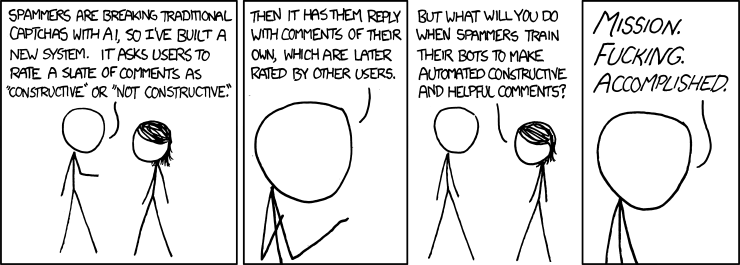
\includegraphics[width=13.75cm]{./img/xkcd-captcha-evolution.png}
	\caption{xkcd on the future of CAPTCHA (Source: \url{http://www.xkcd.com/810/}, accessed on 2013/05/28)}
	\label{fig:xkcdCAPTCHA}
\end{figure}
\begin{figure}
	\centering
	
\includegraphics[width=\textwidth]{./img/reCAPTCHA.png}
	\caption{The reCAPTCHA system (Source: \citep{UNDP2013})}
	\label{fig:reCAPTCHA}
\end{figure}
\begin{figure}
\centering
	\begin{subfigure}[b]{0.49\textwidth}
		\centering
		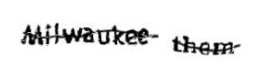
\includegraphics[width=\textwidth]{./img/reCAPTCHA2008.png}
		\caption{Early 2008}
	\end{subfigure}
	\begin{subfigure}[b]{0.49\textwidth}
		\centering
		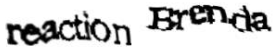
\includegraphics[width=\textwidth]{./img/reCAPTCHA2009.png}
		\caption{December 16th 2009}
	\end{subfigure}
	\begin{subfigure}[b]{0.49\textwidth}
		\centering
		
\includegraphics[width=\textwidth]{./img/reCAPTCHA2010.png}
		\caption{January 24th 2010}
	\end{subfigure}
	\begin{subfigure}[b]{0.49\textwidth}
		\centering
		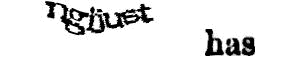
\includegraphics[width=\textwidth]{./img/reCAPTCHA2013.png}
		\caption{May 28th 2013}
	\end{subfigure}
	\caption{Examples of CAPTCHAs directly Downloaded from reCAPTCHA (Source: \citep{Motoyama2010} and \citep{reCAPTCHA2013})}
	\label{fig:captchaEvolution}
\end{figure}
\begin{figure}
\centering
	\begin{subfigure}[b]{0.65\textwidth}
		\centering
		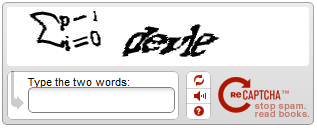
\includegraphics[width=\textwidth]{./img/impossible_captcha01.png}
		\caption{Impossible CAPTCHA (Source: \url{http://asmallpieceofgodsplan.blogspot.be/2012/04/captchas.html} Accessed on 2013-0528)}
	\end{subfigure}
	\begin{subfigure}[b]{0.65\textwidth}
		\centering
		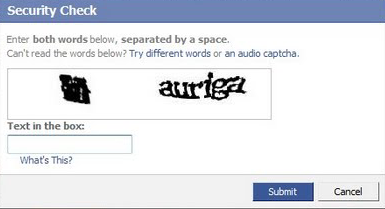
\includegraphics[width=\textwidth]{./img/impossible_captcha02.png}
		\caption{Impossible CAPTCHA (Source: \url{http://asmallpieceofgodsplan.blogspot.be/2012/04/captchas.html} Accessed on 2013-0528)}
	\end{subfigure}
	\begin{subfigure}[b]{0.65\textwidth}
		\centering
		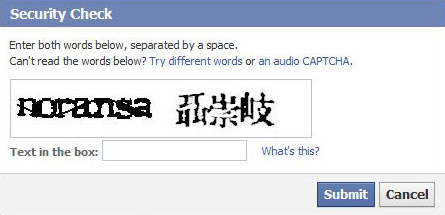
\includegraphics[width=\textwidth]{./img/impossible_captcha03.png}
		\caption{Impossible CAPTCHA (Source: \url{http://oactechnology.com/it-blog/blog/2012/08/31/captcha/} Accessed on 2013-0528)}
	\end{subfigure}
	\begin{subfigure}[b]{0.65\textwidth}
		\centering
		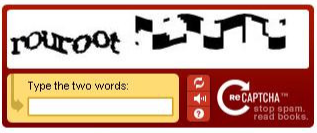
\includegraphics[width=\textwidth]{./img/impossible_captcha04.png}
		\caption{Impossible CAPTCHA (Source: \url{http://ragegenerator.com/pages/comic/39222} Accessed on 2013-0528)}
	\end{subfigure}
	\caption{Examples of CAPTCHAs nearly impossible to solve}
	\label{fig:ImpossibleCaptcha}
\end{figure}
\begin{figure}
	\centering
	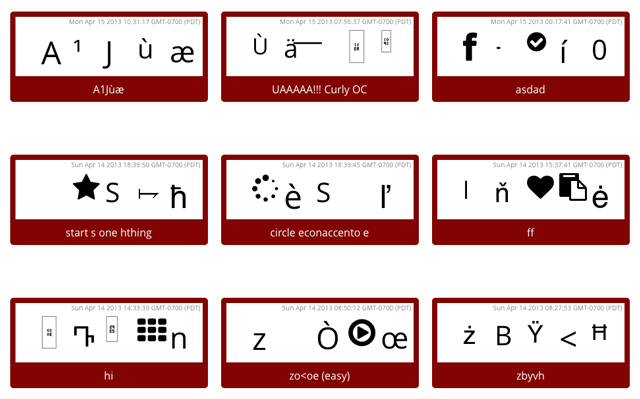
\includegraphics[width=\textwidth]{./img/CRAPCHA.png}
	\caption{Test generated by the CRAPCHA system (Source: \citep{Lsquid2013})}
	\label{fig:CRAPCHA}
\end{figure}
\begin{figure}
	\centering
	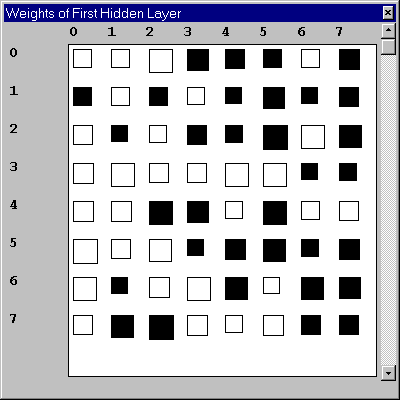
\includegraphics[width=\textwidth]{./img/Hinton_Diagram.png}
	\caption{An example Hinton diagram (Source: \url{http://www.nd.com/products/nsv30/hinton.htm})}
	\label{fig:HintonDiagram}
\end{figure}
\begin{figure}
\centering
	\begin{subfigure}[b]{40px}
	\centering
		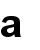
\includegraphics[width=\textwidth]{./img/trainingimages/LATIN_SMALL_LETTER_A-40X50.png}
	\end{subfigure}
	\begin{subfigure}[b]{40px}
	\centering
		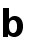
\includegraphics[width=\textwidth]{./img/trainingimages/LATIN_SMALL_LETTER_B-40X50.png}
	\end{subfigure}
	\begin{subfigure}[b]{40px}
	\centering
		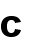
\includegraphics[width=\textwidth]{./img/trainingimages/LATIN_SMALL_LETTER_C-40X50.png}
	\end{subfigure}
	\begin{subfigure}[b]{40px}
	\centering
		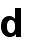
\includegraphics[width=\textwidth]{./img/trainingimages/LATIN_SMALL_LETTER_D-40X50.png}
	\end{subfigure}
	\begin{subfigure}[b]{40px}
	\centering
		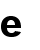
\includegraphics[width=\textwidth]{./img/trainingimages/LATIN_SMALL_LETTER_E-40X50.png}
	\end{subfigure}
	\begin{subfigure}[b]{40px}
	\centering
		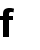
\includegraphics[width=\textwidth]{./img/trainingimages/LATIN_SMALL_LETTER_F-40X50.png}
	\end{subfigure}
	\begin{subfigure}[b]{40px}
	\centering
		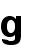
\includegraphics[width=\textwidth]{./img/trainingimages/LATIN_SMALL_LETTER_G-40X50.png}
	\end{subfigure}
	\begin{subfigure}[b]{40px}
	\centering
		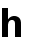
\includegraphics[width=\textwidth]{./img/trainingimages/LATIN_SMALL_LETTER_H-40X50.png}
	\end{subfigure}
	\begin{subfigure}[b]{40px}
	\centering
		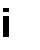
\includegraphics[width=\textwidth]{./img/trainingimages/LATIN_SMALL_LETTER_I-40X50.png}
	\end{subfigure}
	\begin{subfigure}[b]{40px}
	\centering
		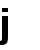
\includegraphics[width=\textwidth]{./img/trainingimages/LATIN_SMALL_LETTER_J-40X50.png}
	\end{subfigure}
	\begin{subfigure}[b]{40px}
	\centering
		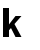
\includegraphics[width=\textwidth]{./img/trainingimages/LATIN_SMALL_LETTER_K-40X50.png}
	\end{subfigure}
	\begin{subfigure}[b]{40px}
	\centering
		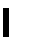
\includegraphics[width=\textwidth]{./img/trainingimages/LATIN_SMALL_LETTER_L-40X50.png}
	\end{subfigure}
	\begin{subfigure}[b]{40px}
	\centering
		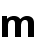
\includegraphics[width=\textwidth]{./img/trainingimages/LATIN_SMALL_LETTER_M-40X50.png}
	\end{subfigure}
	\begin{subfigure}[b]{40px}
	\centering
		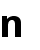
\includegraphics[width=\textwidth]{./img/trainingimages/LATIN_SMALL_LETTER_N-40X50.png}
	\end{subfigure}
	\begin{subfigure}[b]{40px}
	\centering
		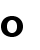
\includegraphics[width=\textwidth]{./img/trainingimages/LATIN_SMALL_LETTER_O-40X50.png}
	\end{subfigure}
	\begin{subfigure}[b]{40px}
	\centering
		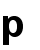
\includegraphics[width=\textwidth]{./img/trainingimages/LATIN_SMALL_LETTER_P-40X50.png}
	\end{subfigure}
	\begin{subfigure}[b]{40px}
	\centering
		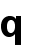
\includegraphics[width=\textwidth]{./img/trainingimages/LATIN_SMALL_LETTER_Q-40X50.png}
	\end{subfigure}
	\begin{subfigure}[b]{40px}
	\centering
		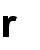
\includegraphics[width=\textwidth]{./img/trainingimages/LATIN_SMALL_LETTER_R-40X50.png}
	\end{subfigure}
	\begin{subfigure}[b]{40px}
	\centering
		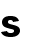
\includegraphics[width=\textwidth]{./img/trainingimages/LATIN_SMALL_LETTER_S-40X50.png}
	\end{subfigure}
	\begin{subfigure}[b]{40px}
	\centering
		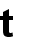
\includegraphics[width=\textwidth]{./img/trainingimages/LATIN_SMALL_LETTER_T-40X50.png}
	\end{subfigure}
	\begin{subfigure}[b]{40px}
	\centering
		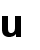
\includegraphics[width=\textwidth]{./img/trainingimages/LATIN_SMALL_LETTER_U-40X50.png}
	\end{subfigure}
	\begin{subfigure}[b]{40px}
	\centering
		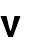
\includegraphics[width=\textwidth]{./img/trainingimages/LATIN_SMALL_LETTER_V-40X50.png}
	\end{subfigure}
	\begin{subfigure}[b]{40px}
	\centering
		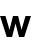
\includegraphics[width=\textwidth]{./img/trainingimages/LATIN_SMALL_LETTER_W-40X50.png}
	\end{subfigure}
	\begin{subfigure}[b]{40px}
	\centering
		\includegraphics[width=\textwidth]{./img/trainingimages/LATIN_SMALL_LETTER_X-40X50.png}
	\end{subfigure}
	\begin{subfigure}[b]{40px}
	\centering
		\includegraphics[width=\textwidth]{./img/trainingimages/LATIN_SMALL_LETTER_Y-40X50.png}
	\end{subfigure}
	\begin{subfigure}[b]{40px}
	\centering
		\includegraphics[width=\textwidth]{./img/trainingimages/LATIN_SMALL_LETTER_Z-40X50.png}
	\end{subfigure}
	\begin{subfigure}[b]{40px}
	\centering
		\includegraphics[width=\textwidth]{./img/trainingimages/DIGIT_ONE-40X50.png}
	\end{subfigure}
	\begin{subfigure}[b]{40px}
	\centering
		\includegraphics[width=\textwidth]{./img/trainingimages/DIGIT_TWO-40X50.png}
	\end{subfigure}
	\begin{subfigure}[b]{40px}
	\centering
		\includegraphics[width=\textwidth]{./img/trainingimages/DIGIT_THREE-40X50.png}
	\end{subfigure}
	\begin{subfigure}[b]{40px}
	\centering
		\includegraphics[width=\textwidth]{./img/trainingimages/DIGIT_FOUR-40X50.png}
	\end{subfigure}
	\begin{subfigure}[b]{40px}
	\centering
		\includegraphics[width=\textwidth]{./img/trainingimages/DIGIT_FIVE-40X50.png}
	\end{subfigure}
	\begin{subfigure}[b]{40px}
	\centering
		\includegraphics[width=\textwidth]{./img/trainingimages/DIGIT_SIX-40X50.png}
	\end{subfigure}
	\begin{subfigure}[b]{40px}
	\centering
		\includegraphics[width=\textwidth]{./img/trainingimages/DIGIT_SEVEN-40X50.png}
	\end{subfigure}
	\begin{subfigure}[b]{40px}
	\centering
		\includegraphics[width=\textwidth]{./img/trainingimages/DIGIT_EIGHT-40X50.png}
	\end{subfigure}
	\begin{subfigure}[b]{40px}
	\centering
		\includegraphics[width=\textwidth]{./img/trainingimages/DIGIT_NINE-40X50.png}
	\end{subfigure}
	\begin{subfigure}[b]{40px}
	\centering
		\includegraphics[width=\textwidth]{./img/trainingimages/DIGIT_ZERO-40X50.png}
	\end{subfigure}
	\begin{subfigure}[b]{40px}
	\centering
		\includegraphics[width=\textwidth]{./img/trainingimages/COMMERCIAL_AT-40X50.png}
	\end{subfigure}
	\begin{subfigure}[b]{40px}
	\centering
		\includegraphics[width=\textwidth]{./img/trainingimages/DOLLAR_SIGN-40X50.png}
	\end{subfigure}
	\begin{subfigure}[b]{40px}
	\centering
		\includegraphics[width=\textwidth]{./img/trainingimages/EQUALS_SIGN-40X50.png}
	\end{subfigure}
	\begin{subfigure}[b]{40px}
	\centering
		\includegraphics[width=\textwidth]{./img/trainingimages/EXCLAMATION_MARK-40X50.png}
	\end{subfigure}
	\begin{subfigure}[b]{40px}
	\centering
		\includegraphics[width=\textwidth]{./img/trainingimages/AMPERSAND-40X50.png}
	\end{subfigure}
	\begin{subfigure}[b]{40px}
	\centering
		\includegraphics[width=\textwidth]{./img/trainingimages/NUMBER_SIGN-40X50.png}
	\end{subfigure}
	\begin{subfigure}[b]{40px}
	\centering
		\includegraphics[width=\textwidth]{./img/trainingimages/PERCENT_SIGN-40X50.png}
	\end{subfigure}
	\begin{subfigure}[b]{40px}
	\centering
		\includegraphics[width=\textwidth]{./img/trainingimages/PLUS_SIGN-40X50.png}
	\end{subfigure}
	\begin{subfigure}[b]{40px}
	\centering
		\includegraphics[width=\textwidth]{./img/trainingimages/QUESTION_MARK-40X50.png}
	\end{subfigure}
\caption{The set of training images}
\label{fig:trainingImages}
\end{figure}
\begin{figure}
\centering
\includegraphics[angle=90,scale=0.45]{./img/perceptron_character_recognition_rate.png}
\caption{Graphical representation of the success rate for perceptron configurations}
\label{fig:PCRR}
\end{figure}
\begin{figure}
\centering
\includegraphics[angle=90,scale=0.45]{./img/Trainingduration.png}
\caption{Graphical representation of the increasing time requirement for training larger networks}
\label{fig:trainingduration}
\end{figure}
\chapter{Tables}
\label{ch:tables}
\begin{sidewaystable}[htbp]
  \centering
  \caption{Overview of the success rate for perceptron configurations}
    \begin{tabular}{rrrrrrrrr}
    \toprule
    Configuration & Accuracy & evaluation & evaluation \% & normal & normal \% & distroted & distorted \% & trainingduration \\
    \midrule
    \multicolumn{1}{c}{\multirow{3}[0]{*}{2000-8}} & 10\%  & 50    & 46,30\% & 69    & 13,80\% & 74    & 14,80\% & 0,22 \\
    \multicolumn{1}{c}{} & 1\%   & 105   & 97,22\% & 93    & 18,60\% & 79    & 15,80\% & 0,34 \\
    \multicolumn{1}{c}{} & 0,10\% & 108   & 100,00\% & 32    & 6,40\% & 90    & 18,00\% & 0,47 \\
    \multicolumn{1}{c}{\multirow{3}[0]{*}{2000-500-8}} & 10\%  & 48    & 44,44\% & 46    & 9,20\% & 28    & 5,60\% & 42,45 \\
    \multicolumn{1}{c}{} & 1\%   & 102   & 94,44\% & 75    & 15,00\% & 43    & 8,60\% & 63,8 \\
    \multicolumn{1}{c}{} & 0,10\% & 108   & 100,00\% & 59    & 11,80\% & 54    & 10,80\% & 76,22 \\
    \multicolumn{1}{c}{\multirow{3}[0]{*}{2000-1000-8}} & 10\%  & 32    & 29,63\% & 73    & 14,60\% & 80    & 16,00\% & 86,98 \\
    \multicolumn{1}{c}{} & 1\%   & 103   & 95,37\% & 24    & 4,80\% & 36    & 7,20\% & 120,96 \\
    \multicolumn{1}{c}{} & 0,10\% & 108   & 100,00\% & 87    & 17,40\% & 50    & 10,00\% & 145,82 \\
    \multicolumn{1}{c}{\multirow{3}[0]{*}{2000-1500-8}} & 10\%  & 45    & 41,67\% & 30    & 6,00\% & 27    & 5,40\% & 137,53 \\
    \multicolumn{1}{c}{} & 1\%   & 105   & 97,22\% & 18    & 3,60\% & 36    & 7,20\% & 207,33 \\
    \multicolumn{1}{c}{} & 0,10\% & 108   & 100,00\% & 103   & 20,60\% & 35    & 7,00\% & 230,98 \\
    \multicolumn{1}{c}{\multirow{3}[0]{*}{2000-2000-8}} & 10\%  & 49    & 45,37\% & 75    & 15,00\% & 11    & 2,20\% & 189,4 \\
    \multicolumn{1}{c}{} & 1\%   & 104   & 96,30\% & 34    & 6,80\% & 46    & 9,20\% & 262,35 \\
    \multicolumn{1}{c}{} & 0,10\% & 108   & 100,00\% & 110   & 22,00\% & 27    & 5,40\% & 305,6 \\
    \multicolumn{1}{c}{\multirow{3}[0]{*}{2000-2500-8}} & 10\%  & 41    & 37,96\% & 40    & 8,00\% & 29    & 5,80\% & 238,29 \\
    \multicolumn{1}{c}{} & 1\%   & 100   & 92,59\% & 62    & 12,40\% & 41    & 8,20\% & 343,44 \\
    \multicolumn{1}{c}{} & 0,10\% & 108   & 100,00\% & 54    & 10,80\% & 43    & 8,60\% & 381,68 \\
    \multicolumn{1}{c}{\multirow{3}[0]{*}{2000-3000-8}} & 10\%  & 43    & 39,81\% & 44    & 8,80\% & 22    & 4,40\% & 301,65 \\
    \multicolumn{1}{c}{} & 1\%   & 105   & 97,22\% & 61    & 12,20\% & 50    & 10,00\% & 412,99 \\
    \multicolumn{1}{c}{} & 0,10\% & 108   & 100,00\% & 39    & 7,80\% & 17    & 3,40\% & 445,79 \\
    \multicolumn{1}{c}{\multirow{3}[0]{*}{2000-3500-8}} & 10\%  & 38    & 35,19\% & 17    & 3,40\% & 40    & 8,00\% & 334,87 \\
    \multicolumn{1}{c}{} & 1\%   & 103   & 95,37\% & 45    & 9,00\% & 54    & 10,80\% & 461,98 \\
    \multicolumn{1}{c}{} & 0,10\% & 108   & 100,00\% & 91    & 18,20\% & 24    & 4,80\% & 520,07 \\
    \multicolumn{1}{c}{\multirow{3}[0]{*}{2000-4000-8}} & 10\%  & 30    & 27,78\% & 24    & 4,80\% & 34    & 6,80\% & 380,71 \\
    \multicolumn{1}{c}{} & 1\%   & 103   & 95,37\% & 64    & 12,80\% & 39    & 7,80\% & 531,18 \\
    \multicolumn{1}{c}{} & 0,10\% & 108   & 100,00\% & 51    & 10,20\% & 11    & 2,20\% & 613,68 \\
    \multicolumn{1}{c}{\multirow{3}[0]{*}{2000-4500-8}} & 10\%  & 58    & 53,70\% & 73    & 14,60\% & 0     & 0,00\% & 498,38 \\
    \multicolumn{1}{c}{} & 1\%   & 102   & 94,44\% & 41    & 8,20\% & 7     & 1,40\% & 621,92 \\
    \multicolumn{1}{c}{} & 0,10\% & 106   & 98,15\% & 76    & 15,20\% & 29    & 5,80\% & 713,27 \\
    \bottomrule
    \end{tabular}%
  \label{tab:PCRR}%
\end{sidewaystable}

\cleardoublepage
\bibliographystyle{plainnat}
\bibliography{Solving_CAPTCHA_using_neural_networks}
%
%%---------- Back matter -------------------------------------------------
%
\cleardoublepage

\listoffigures
\listoftables

\cleardoublepage
% Lijst van broncode-listings. Kan je weglaten als je dit niet nodig hebt.
\lstlistoflistings
%

\cleardoublepage
\chapter{CD}
\label{ch:cd}
\end{document}